\documentclass[journal]{IEEEtran}

\usepackage{amsmath,amssymb,amsfonts}
\usepackage{bm}
\usepackage{cite}
\usepackage{graphicx}
\usepackage{booktabs}
\usepackage{array}
\usepackage{url}
\usepackage{xcolor}
\usepackage{algorithm}
\usepackage{algorithmic}

\newtheorem{proposition}{Proposition}
\newtheorem{theorem}{Theorem}
\newtheorem{lemma}{Lemma}
\newtheorem{remark}{Remark}

\newcommand{\R}{\mathbb{R}}
\newcommand{\C}{\mathbb{C}}
\newcommand{\Lt}{\widetilde L}
\newcommand{\Dt}{\widetilde D}
\newcommand{\zt}{\zeta}
\newcommand{\nus}{\nu}
\newcommand{\diag}{\operatorname{diag}}
\newcommand{\Real}{\operatorname{Re}}
\newcommand{\Imag}{\operatorname{Im}}
\newcommand{\argmin}{\operatorname*{arg\,min}}
\newcommand{\argmax}{\operatorname*{arg\,max}}
\newcommand{\norm}[1]{\left\lVert #1 \right\rVert}

\title{Controller-Aware Rational Self-Energy for Damping-Margin Analysis of IBR Grids}

\author{Jorge L. Mayorga Taborda%
\thanks{J. L. Mayorga Taborda is with Universidad de los Andes, Bogota, Colombia. E-mail: author@example.com.}%
\thanks{This manuscript is a pre-submission research draft. The method, synthetic stress tests, reduced PLL tests, and an ANDES controller-aware bridge validation are reported explicitly; full estimator and planning validation over calibrated ANDES IBR operating ranges remains required before any final journal submission.}}

\markboth{IEEE Transactions Manuscript Draft, June 2026}%
{Mayorga Taborda: Controller-Aware Self-Energy for IBR Damping Margins}

\begin{document}

\maketitle

\begin{abstract}
The replacement of synchronous generation by inverter-based resources changes not only grid inertia but also the location of damping itself. In detailed small-signal models, much of the observed damping can be supplied by controller, exciter, stabilizer, PLL, and inverter states rather than by a static nodal damping coefficient. This paper argues that the appropriate reduced object for such systems is therefore not a constant-coefficient scalar QEP, but a controller-aware rational self-energy,
\[
\Sigma(s)=D_0+C(sI-A_{cc})^{-1}B,
\]
or, equivalently, a Schur nonlinear eigenvalue problem (NEP) for the retained network/interface states. The main full-ANDES result is a bridge audit on IEEE 39-bus cases: the static scalar bridge fails because \texttt{GENROU.D}=0 does not contain the measured modal damping, while the rational Schur NEP solved by Beyn contour integration extracts the same critical poles as the full ANDES eigensolve in no-PSS, packaged-base, and Mix60 SG-to-IBR cases. In Mix60, the bridge captures a 13.7 Hz PLL-family critical mode with $\pi_c=0.853$ that is missed by both the scalar bridge and a fixed-point Schur iteration. This bridge separates network-family and control-family criticality and enables mechanism audits without discarding controller dynamics. Around network-family modes, the paper also develops a second-order modal perturbation and rational graph-filter interpretation of non-proportional damping. Synthetic and reduced-PLL tests show where this correction improves a diagonal damping-region screen and where reduced-QEP fallback remains necessary; full estimator and planning validation over the controller-aware bridge remain the next registered experiments. The bridge also reveals a modal-local control-resonant reinforcement reversal: in a minority of Mix60/no-PSS line tests, strengthening a line moves a network-family mode toward a PLL-dominated condensed-control pole and the self-energy term sets the damping decrease; the mechanism disappears under a soft-GFL negative control. Finally, an input--output extension derives a protected-resolvent graph-filter sensitivity that gives a common local exchange rate for topology, damping, inertia, and controller actions. Reduced-model gates show robust disagreement between modal damping rankings and protected-resolvent rankings and support coordinated $w+D$ and $w+M$ packages as candidates; those claims remain pending full ANDES flow-feasible validation.
\end{abstract}

\begin{IEEEkeywords}
Damping ratio, inverter-based resources, eigenvalue perturbation, phase-locked loop, quadratic eigenvalue problem, rational graph filter, graph signal processing, small-signal stability.
\end{IEEEkeywords}

\section{Introduction}

Power systems are moving from synchronous-machine-dominated dynamics toward networks with high penetration of inverter-based resources (IBRs). The most visible effect of this transition is reduced inertia, but the more difficult small-signal effect is that damping is no longer proportional to inertia or to network stiffness. A synchronous generator contributes inertia and damping through electromechanical dynamics. A grid-following inverter contributes control damping through a phase-locked loop and current controller; a grid-forming inverter contributes droop or virtual-synchronous-machine behavior. These mechanisms are physically different and appear in the linearized model as heterogeneous, non-commuting dynamic coefficients.

The standard swing-equation intuition says that low-frequency inter-area modes are critical and that increasing network stiffness improves robustness. Those statements are useful but incomplete. The damping ratio of a mode is not simply a graph frequency. If a line reinforcement raises the oscillation frequency without increasing the modal decay rate enough, the damping ratio can decrease. Likewise, if damping is heterogeneous, the mode with lowest damping ratio need not be the Fiedler mode or the highest-frequency mode. Planning rules based only on $\lambda_2$, Fiedler participation, or frequency sensitivities can therefore be misleading in an IBR-rich grid.

This paper asks a narrow question: what reduced spectral object preserves the damping-margin mechanisms of an IBR grid after controller states are condensed? The answer proposed here is a controller-aware rational self-energy. A static scalar damping coefficient is sufficient only when the condensed dynamics can be represented at the relevant frequency by a constant term. In the ANDES cases studied here, that condition fails: damping is supplied largely by controller and auxiliary states, so the reduced object must remain frequency dependent.

The central message is not that a new graph eigenvalue replaces small-signal analysis. The central message is that a rational Schur bridge preserves controller-mediated damping mechanisms that a static $(L,M,D)$ bridge loses. Once that bridge is available, lower-order spectral perturbations can be used as interpretable screens, but they must be checked against the complete NEP or full eigensolve when controller resonances or clustered modes are present.

The paper makes three calibrated methodological contributions and two mechanism/bridge findings. The novelty claim is at the level of power-system formulation, interpretation, and validated mechanism, not at the level of inventing eigenvalue perturbation theory or contour eigensolvers.

\begin{itemize}
\item It shows, on reproducible IEEE 39-bus ANDES cases, that a static scalar $(L,M,D)$ bridge can fail because controller and auxiliary states carry the observed damping. The controller-aware rational Schur NEP is the reduced object that retains those effects.
\item It solves that NEP by contour integration and classifies extracted zeros into network-family and control-family modes using condensed-state participation. This recovers the Mix60 13.7 Hz PLL-family critical pole missed by scalar and fixed-point reductions.
\item It uses the damping-region plane $(\nu_k,\delta_k)$ as the zero-order network picture. This is an interpretive coordinate system for heterogeneous IBR damping, not a claim that the proportional modal formula is new.
\item It derives and tests a closed-form second-order correction for the critical damping-margin pole under off-diagonal modal damping. This correction explains, term by term, how non-proportional inverter damping couples the critical mode to other modes.
\item It organizes the estimator as a diagnostic workflow: diagonal screen, second-order correction, and reduced-QEP fallback for clustered or strongly coupled regimes. The negative cases where second order worsens the tail are part of the method, because they justify the trigger; full-ANDES estimator validation remains a registered next experiment.
\item It uses the bridge to identify a control-resonant reinforcement reversal: a line action can pull a network-family mode toward a PLL-dominated condensed-control pole, so the self-energy term drives a damping decrease. This is reported as a modal-local mechanism with a negative control, not as a universal Braess paradox.
\item It derives a protected-resolvent graph-filter sensitivity for non-normal IBR grids. This input--output certificate is separate from the damping-ratio pole metric and exposes spatial decoupling between forcing and response. Current evidence supports it as a reduced-model planning candidate, not yet as a full-ANDES flow-feasible planner.
\end{itemize}

\noindent\textbf{Unified spectral-attribution object.}
All pieces of the paper are organized by the same retained-network NEP,
\begin{equation}
T(s)=s^2M+s\Sigma(s)+\Lt,\qquad
\Sigma(s)=D_0+C(sI-A_{cc})^{-1}B .
\label{eq:intro_unified_object}
\end{equation}
This operator is used as an attribution ledger. The network lever is $\Lt$, the inertia or virtual-mass lever is $M$, and the controller lever is the rational self-energy $\Sigma(s)$. A damping-margin claim is therefore not accepted because one score is large; it must specify which lever moved the pole, which competing explanation was controlled, and whether the reduced prediction agrees with the full NEP or full ANDES eigensolve. In this ledger, the static damping-region screen is the zero-order network picture, the second-order correction is the local modal-coupling picture, the Schur self-energy is the controller-aware full bridge, and the reinforcement audit is a pole-sensitivity mechanism test. The possible inertia--control cross term is retained as local theory, but the initial Phase-E0 ANDES tests found $0/13$ measurable singleton GENROU--PLL cross cases; it is therefore not used as the empirical headline of this draft.

The present manuscript is deliberately calibrated. Proportional modal damping, Rayleigh sensitivity, QEP sensitivity, contour NEP solvers, Schur complements, and eigenvalue perturbation are established tools. The candidate contribution is to assemble them into a controller-aware damping-margin bridge for IBR grids, document why the static scalar bridge fails, and use the retained self-energy to expose network-family versus control-family mechanisms. Synthetic stress tests and a reduced PLL model are reported to identify how a cheap second-order estimator behaves. The IEEE 39-bus ANDES evidence validates the rational bridge and one bridge-enabled mechanism audit. It does not by itself validate the full estimator, conversion-ranking, or planning claims.

\section{Related Work}

Small-signal power-system stability is a mature field; standard references include modal analysis of electromechanical oscillations and damping-ratio sensitivity \cite{kundur1994power,rogers2000oscillations}. Spectral and system-theoretic approaches to power networks have clarified the role of Laplacian eigenvalues, inertia, and damping in low-inertia performance \cite{pirani2017system,paganini2017global,pagnier2019optimal}. In the proportional or homogeneous case, modal frequencies scale as $\sqrt{\nu_k}$ and damping ratios take a closed form involving damping, inertia, and graph eigenvalues. Those results are essential background for this paper rather than its novelty.

IBR-dominated systems complicate this picture because their controls introduce additional states, time scales, and non-proportional damping. Recent small-signal studies of inverter networks emphasize the role of line dynamics, operating conditions, and converter-control parameters \cite{henriquez2022load,kravis2023inverter,nishino2025closed}. Stability-region and security-region viewpoints for converter-dominated systems are also active research topics \cite{conte2026stability,lai2026switching}. This activity creates both an opportunity and a risk: region language is useful, but broad claims of originality are unsafe unless the exact reduced spectral construction is differentiated carefully.

The proposed damping-region picture is inspired by consensus-region theory in multi-agent systems. In that literature, stability of a networked linear system can be tested by asking whether scaled nonzero Laplacian eigenvalues lie in a region determined by local agent dynamics and feedback gains \cite{li2014consensus}. Related networked-control books develop dynamic topologies, switching graphs, dwell-time logic, resilient consensus, delays, and event-triggered control \cite{wen2021dynamic,ding2022microgrids}. The present paper does not import those results wholesale. A power grid with IBR controls is not a first-order consensus system. The transfer is conceptual: define the region induced by local dynamics and use graph-modal coordinates to screen network-level stability.

Quadratic eigenvalue problems provide the natural algebraic language for second-order small-signal models \cite{tisseur2001qep}. If damping and stiffness commute, the QEP decouples into scalar modal equations. If not, modes are coupled through off-diagonal modal damping terms. Modal perturbation for non-proportionally damped systems is well established in structural dynamics \cite{pan2020modal,conde2021nonproportionality}; this paper does not claim that perturbation theory itself is new. The proposed distinction is the power-system use of the second-order term as a damping-margin decomposition and as a rational graph filter of $(\Lt,\Dt)$.

Planning-oriented damping metrics also have nearby prior art. Grid-forming inverter placement by composite frequency and damping indices has been studied on modified IEEE 39-bus systems \cite{liyanage2025gfmi}. Closed-form damping-ratio sensitivities based on QEP formulations have also been derived for power-system remedial actions \cite{setareh2025damping}. The line-reinforcement and weak-node maps in this manuscript must therefore be read as applications of the proposed margin object and must be compared against these baselines. The validation platform used here is ANDES, an open-source symbolic-numeric power-system modeling tool with power flow, time-domain, and eigenvalue analysis \cite{cui2021andes,andesdocs}.

\begin{table*}[t]
\centering
\caption{Nearest prior art and novelty boundary. The paper does not claim novelty for generic perturbation theory, QEP sensitivity, or damping-ratio placement metrics.}
\label{tab:priorart}
\scriptsize
\begin{tabular}{@{}p{0.19\textwidth}p{0.26\textwidth}p{0.24\textwidth}p{0.22\textwidth}@{}}
\toprule
Reference area & What is already established & What is not claimed here & Candidate distinction here\\
\midrule
Non-proportional modal perturbation \cite{pan2020modal,conde2021nonproportionality}
& Perturbation methods and indices for non-classically damped second-order systems.
& The perturbation expansion itself is not new.
& Use the second-order term as a damping-margin decomposition for IBR grids and express it as a rational filter of $(\Lt,\Dt)$.\\
GFM placement by stability indices \cite{liyanage2025gfmi}
& Placement/ranking of grid-forming inverters on modified IEEE 39 cases using frequency and damping-related indices.
& Ranking inverter placement by a damping metric is not new.
& Compare conversion decisions using the proposed margin estimator and report regret against full eigensolve baselines.\\
QEP damping-ratio sensitivities \cite{setareh2025damping}
& Closed-form QEP sensitivities for damping-ratio remedial actions in synchronous-generator models.
& QEP sensitivity formulas are not new.
& Apply damping-ratio sensitivity to line reinforcement and IBR-oriented margin maps, with frequency-only ranking as a negative control.\\
\bottomrule
\end{tabular}
\end{table*}

\section{Network Model and Damping Region}

Consider a lossless small-signal power network linearized around an operating point:
\begin{equation}
M\ddot{\theta}+D\dot{\theta}+L\theta=p,
\label{eq:swing}
\end{equation}
where $M=\diag(M_i)\succ0$, $D=\diag(D_i)\succeq0$, and $L$ is the weighted Laplacian induced by the active-power Jacobian. In the usual approximation,
\begin{equation}
L_{ij}=-V_iV_jb_{ij}\cos(\theta_i^\star-\theta_j^\star),\quad i\neq j,
\end{equation}
with diagonal entries chosen so that $L\mathbf{1}=0$. The analysis is performed in inertia-normalized coordinates $\vartheta=M^{1/2}\theta$, giving
\begin{equation}
\ddot{\vartheta}+\Dt\dot{\vartheta}+\Lt\vartheta=M^{-1/2}p,
\label{eq:normalized}
\end{equation}
where
\begin{equation}
\Lt=M^{-1/2}LM^{-1/2},\qquad \Dt=M^{-1/2}DM^{-1/2}.
\end{equation}
Let $\Lt q_k=\nu_kq_k$, with $Q=[q_1,\ldots,q_n]$ orthonormal. The zero eigenvalue associated with uniform angle shift is discarded. In modal coordinates $x=Q^T\vartheta$, the dynamics are
\begin{equation}
\ddot{x}+\Gamma\dot{x}+\Lambda x=Q^TM^{-1/2}p,
\label{eq:modal}
\end{equation}
where $\Gamma=Q^T\Dt Q$ and $\Lambda=\diag(\nu_k)$. The diagonal entries
\begin{equation}
\delta_k=\Gamma_{kk}=q_k^T\Dt q_k
\end{equation}
are modal damping coefficients, while the off-diagonal entries $\Gamma_{\ell k}$ describe damping-induced modal coupling.

The exact small-signal poles are roots of the QEP
\begin{equation}
P(s)v=(s^2I+s\Dt+\Lt)v=0.
\label{eq:qep}
\end{equation}
Equivalently, they are eigenvalues of the first-order matrix
\begin{equation}
A=\begin{bmatrix}
0&I\\
-M^{-1}L&-M^{-1}D
\end{bmatrix}.
\end{equation}
The damping margin is
\begin{equation}
\zeta_{\min}=\min_{s_j\in\mathcal{S}_{\rm osc}}\frac{-\Real(s_j)}{|s_j|},
\label{eq:zeta}
\end{equation}
where $\mathcal{S}_{\rm osc}$ contains complex oscillatory poles.

\subsection{Damping Region}

If $\Lt$ and $\Dt$ commute, then $\Gamma$ is diagonal and each nonzero mode solves
\begin{equation}
s^2+\delta_ks+\nu_k=0.
\end{equation}
For an underdamped mode,
\begin{equation}
\zeta_k=\frac{\delta_k}{2\sqrt{\nu_k}}.
\label{eq:diagzeta}
\end{equation}
Thus a target damping margin $\zeta_\star$ is equivalent to
\begin{equation}
\delta_k\geq 2\zeta_\star\sqrt{\nu_k},\qquad k=2,\ldots,n.
\label{eq:region}
\end{equation}
Equation \eqref{eq:region} defines the damping region shown in Fig.~\ref{fig:region}. Modes below the curve violate the target damping margin. Modes above it satisfy the target in the proportional case.

\begin{figure}[t]
\centering
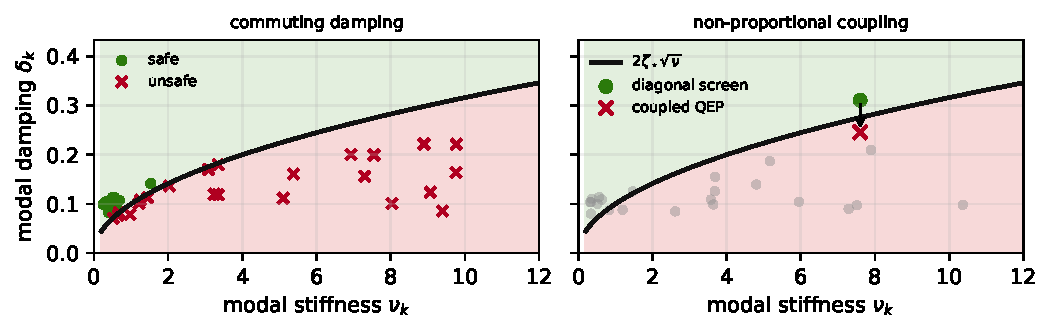
\includegraphics[width=\columnwidth]{figures/fig1_damping_region.pdf}
\caption{Damping-region view. Left: in the commuting case, a target $\zeta_\star$ becomes the exact boundary $\delta=2\zeta_\star\sqrt{\nu}$. Right: in non-proportional damping, a diagonal modal point can appear safe while QEP coupling moves the pole below the margin. The region is therefore a screen, not a certificate, outside the commuting regime.}
\label{fig:region}
\end{figure}

This region should not be overinterpreted. In the non-proportional case, $\Gamma$ is not diagonal, and \eqref{eq:diagzeta} is no longer exact. It remains a first-order approximation when damping is weak and modal frequencies are well separated. It can fail when low-damping modes are clustered or when $\Gamma_{\ell k}$ is large relative to the modal frequency separation. This observation motivates an adaptive estimator rather than a single formula.

\begin{proposition}[Exact region in the commuting case]
Suppose $\Lt$ and $\Dt$ are symmetric and share an orthonormal eigenbasis on the nonzero-angle subspace. Then the damping margin of \eqref{eq:normalized} is
\begin{equation}
\zeta_{\min}=\min_{\nu_k>0}\frac{\delta_k}{2\sqrt{\nu_k}},
\end{equation}
provided the limiting modes are underdamped. Moreover, a target margin $\zeta_\star$ is satisfied if and only if every nonzero modal point obeys
\begin{equation}
\delta_k\geq 2\zeta_\star\sqrt{\nu_k}.
\end{equation}
\end{proposition}

The proof follows by diagonalizing both matrices in \eqref{eq:normalized}. It is stated explicitly because it fixes the boundary of the proposed framework. The region is exact only when damping is diagonal in the graph-modal basis. In every other case, the same inequality is a screen, not a certificate.

\begin{proposition}[First-order modal-coupling warning]
Let $\nu_k$ and $\nu_\ell$ be two distinct inertial-Laplacian eigenvalues and let $\Gamma_{\ell k}\neq0$. The sensitivity of modal damping to a perturbation that rotates $q_k$ toward $q_\ell$ scales with
\begin{equation}
\frac{\Gamma_{\ell k}}{\nu_k-\nu_\ell}.
\end{equation}
Thus clustered graph frequencies and large off-diagonal modal damping are the cases in which the diagonal region is least reliable.
\end{proposition}

This warning is diagnostic, not a replacement for the full QEP. It explains why two networks with the same diagonal modal points can have different damping margins: the missing information is the coupling geometry in $Q^T\Dt Q$, weighted by modal separation. This is the mechanism behind the adaptive estimator in the next section.

\begin{remark}[Critical mode selection]
For damping ratio, the critical graph mode is not generically the Fiedler mode. In proportional damping with homogeneous damping per inertia, the smallest damping ratio may be controlled by the largest $\nu_k$ because $\zeta_k$ scales like $1/\sqrt{\nu_k}$. In heterogeneous IBR cases, the critical mode is determined by the pair $(\nu_k,\delta_k)$ and by modal coupling. Any benchmark that compares only the Fiedler-mode estimate against the full eigensolve is therefore using the wrong control.
\end{remark}

\section{Adaptive Spectral Margin Estimator}

The estimator uses the diagonal region as a cheap screen, a second-order perturbation as the closed-form correction, and the reduced QEP as a fallback. The diagonal all-mode estimate is
\begin{equation}
\widehat{\zeta}_{\rm diag}=\min_{k:\nu_k>0}\frac{q_k^T\Dt q_k}{2\sqrt{\nu_k}}.
\label{eq:zdiag}
\end{equation}
This is not the Fiedler-mode estimate. It takes the minimum over all modes. In homogeneous damping the critical mode is often the largest-frequency mode; in heterogeneous damping it need not be.

\subsection{Closed-Form Second-Order Correction}

Let $\Gamma=\Delta+E$, where $\Delta=\diag(\delta_k)$ and $E$ contains the off-diagonal modal damping. The zero-order diagonal pole of the critical mode $c$ is $s_0$, where
\begin{equation}
s_0^2+\delta_cs_0+\nu_c=0.
\end{equation}
Let $p_\ell(s)=s^2+\delta_\ell s+\nu_\ell$. Partition the modal coordinates into the critical coordinate $z_c$ and all remaining coordinates $z_R$. To second order in the off-diagonal damping, the coupled modal equations are
\begin{align}
p_c(s)z_c+sE_{cR}z_R&=0,\\
\diag(p_\ell(s))z_R+sE_{Rc}z_c&=0,
\end{align}
where the $E_{RR}$ block would contribute only higher-order terms to the scalar critical equation. Thus
\begin{equation}
z_R=-s\,\diag(p_\ell(s))^{-1}E_{Rc}z_c+O(\|E\|^2).
\end{equation}
Substitution into the critical equation gives
\begin{equation}
p_c(s)-s^2E_{cR}\diag(p_\ell(s))^{-1}E_{Rc}=0+O(\|E\|^3).
\end{equation}
Writing $s=s_0+\Delta s_c$ and evaluating the resolvent at the critical pole $s_0$ yields the second-order pole correction
\begin{equation}
\Delta s_c=
\frac{s_0^2}{2s_0+\delta_c}
\sum_{\ell\neq c}
\frac{E_{c\ell}E_{\ell c}}
{s_0^2+\delta_\ell s_0+\nu_\ell}.
\label{eq:secondorder}
\end{equation}
The corrected pole is $s_c^{(2)}=s_0+\Delta s_c$ and the corrected margin is
\begin{equation}
\widehat{\zeta}_{2}=-\frac{\Real(s_c^{(2)})}{|s_c^{(2)}|}.
\label{eq:zeta2}
\end{equation}
Equation \eqref{eq:secondorder} is the central estimator in this manuscript. It is not a new perturbation theorem; it is a power-system use of second-order eigenvalue perturbation to quantify how non-proportional inverter damping moves the critical damping-margin pole away from the diagonal network prediction.

\subsection{Joint Inertia--Damping Perturbation}

The previous correction assumes that $\Lt$ is fixed and that only off-diagonal modal damping perturbs the diagonal QEP. A finite SG-to-IBR conversion, however, changes both inertia and damping. Let a small conversion parameter $\rho$ define
\begin{equation}
M(\rho)=M_0+\rho\Delta M,\qquad
D(\rho)=D_0+\rho\Delta D,
\end{equation}
and define
\begin{equation}
\Lambda_1=Q^T\frac{d\Lt}{d\rho}Q,\qquad
\Gamma_1=Q^T\frac{d\Dt}{d\rho}Q
\end{equation}
in the unperturbed inertial-Laplacian basis. The first-order shift of the critical diagonal pole is
\begin{equation}
s_1=-\frac{\Lambda_{1,cc}+s_0\Gamma_{1,cc}}{2s_0+\delta_c}.
\label{eq:jointfirst}
\end{equation}
The local pole approximation has the form
\begin{equation}
s_c=s_0+s_1+s_{2,{\rm coup}}+\hbox{diagonal self terms}+O(\rho^3).
\end{equation}
The next equation isolates only the modal-coupling part of the second-order term; it is not the complete finite-conversion pole shift.
The off-diagonal second-order coupling contribution is obtained by replacing the perturbation $sE$ in \eqref{eq:secondorder} with the combined channel
\begin{equation}
H_1(s_0)=s_0\Gamma_1+\Lambda_1.
\end{equation}
Thus
\begin{align}
s_{2,{\rm coup}}
&=\frac{1}{2s_0+\delta_c}
\sum_{\ell\neq c}
\frac{N_{c\ell}(s_0)}
{s_0^2+\delta_\ell s_0+\nu_\ell},
\label{eq:jointsecond}\\
N_{c\ell}(s_0)
&=\left(s_0E^{(D)}_{c\ell}+E^{(L)}_{c\ell}\right)
\left(s_0E^{(D)}_{\ell c}+E^{(L)}_{\ell c}\right).
\end{align}
where $E^{(D)}=\operatorname{offdiag}(\Gamma_1)$ and
$E^{(L)}=\operatorname{offdiag}(\Lambda_1)$. If $\Delta M=0$, then
$E^{(L)}=0$ and \eqref{eq:jointsecond} collapses to \eqref{eq:secondorder}. Expanding the numerator exposes the non-additive term
\begin{equation}
s_0\left(
E^{(D)}_{c\ell}E^{(L)}_{\ell c}
+E^{(L)}_{c\ell}E^{(D)}_{\ell c}
\right),
\label{eq:cross}
\end{equation}
which is the explicit red-control interaction: damping and inertia perturbations do not generally move the critical pole as two separable scalar effects.

Equation \eqref{eq:jointsecond} is used here as a mechanism statement and as a local score for small virtual-inertia or droop retuning. It should not be presented as a reliable estimator for a large finite SG-to-IBR conversion. For such conversions, the adaptive estimator or the full model must be recomputed after each candidate action. The full second-order expansion also contains scalar self terms from the diagonal first-order shift $s_1$; \eqref{eq:jointsecond} isolates the modal-coupling contribution that generalizes the rational-filter correction.

\subsection{Rational Graph-Filter Form}

The same correction can be written in graph-signal-processing language. A polynomial filter of the inertial Laplacian,
\begin{equation}
h(\Lt)=\sum_{m=0}^{M_h} a_m \Lt^m,
\end{equation}
acts diagonally in the eigenbasis of $\Lt$: $h(\Lt)q_k=h(\nu_k)q_k$. It can rescale modal components, but it cannot create the off-diagonal modal damping entries that are absent from a graph-frequency-only description. This is the structural reason why a polynomial filter of $\Lt$ alone is not a damping-margin model for a non-proportionally damped IBR grid.

Define the pole-dependent rational filter
\begin{equation}
H(\Lambda;s_0)=\diag\left(\frac{1}{s_0^2+\delta_\ell s_0+\nu_\ell}\right)_{\ell\neq c},
\end{equation}
with the critical index omitted from the diagonal action. Then \eqref{eq:secondorder} is equivalently
\begin{equation}
\Delta s_c=
\frac{s_0^2}{2s_0+\delta_c}
\left[E H(\Lambda;s_0) E\right]_{cc}.
\label{eq:rationalfilter}
\end{equation}

\begin{proposition}[Rational pair-filter interpretation]
The second-order margin correction is a rational filter of the dynamic operator pair $(\Lt,\Dt)$ evaluated at the diagonal critical pole. It depends on $\Lt$ through the modal frequencies $\nu_\ell$, on $\Dt$ through $\delta_\ell$ and $E=\operatorname{offdiag}(Q^T\Dt Q)$, and on the dynamics through $s_0$. It is therefore not reducible to a polynomial filter of $\Lt$.
\end{proposition}

\emph{Proof:}
Equation \eqref{eq:secondorder} can be factored by collecting the modal denominators into the diagonal operator $H(\Lambda;s_0)$. The left and right multiplications by $E$ inject and recover the non-proportional damping coupling. If $E=0$, the filter output is zero and the proportional damping-region formula is exact. If $E\neq0$, the correction weights each coupled mode by its resolvent-like separation from the critical pole. \hfill$\square$

This filter form is an interpretation of \eqref{eq:secondorder}, not a second independent mechanism. Its value is that it states precisely what graph information is missing from $\Lt$ alone: damping margin is governed by the pair $(\Lt,\Dt)$ and by the pole at which the pair is evaluated.

The correction is used only when the perturbation is credible. If $|s_0^2+\delta_\ell s_0+\nu_\ell|$ is small for a neighboring mode, or if $|\Delta s_c|$ is comparable to $|s_0|$, the method should reject the correction and solve a reduced QEP instead.

Define a simple coupling score for a candidate mode set $\mathcal{I}$:
\begin{equation}
\eta(\mathcal{I})=\max_{\substack{k,\ell\in\mathcal{I}\\k\neq \ell}}
\frac{|\Gamma_{\ell k}|}{|\sqrt{\nu_\ell}-\sqrt{\nu_k}|+\epsilon},
\label{eq:eta}
\end{equation}
where $\epsilon>0$ prevents division by zero. Large $\eta$ indicates that modal damping couples frequencies too strongly for a purely diagonal approximation. More elaborate diagnostics can include the coupling to nearby modes outside $\mathcal{I}$ and the residual of the reduced QEP.

Let $\mathcal{I}_r$ contain the modes with the smallest diagonal damping estimates and any neighboring modes triggered by \eqref{eq:eta}. With $V=Q[:,\mathcal{I}_r]$, form
\begin{equation}
L_r=V^T\Lt V,\qquad D_r=V^T\Dt V,
\end{equation}
and solve
\begin{equation}
(s^2I_r+sD_r+L_r)w=0.
\label{eq:rqep}
\end{equation}
The adaptive estimate returns the diagonal estimate when the coupling diagnostic is small and the reduced-QEP estimate otherwise.

\begin{algorithm}[t]
\caption{Adaptive damping-margin estimator}
\label{alg:adaptive}
\begin{algorithmic}[1]
\STATE Input: $L,M,D$, reduced size $r$, thresholds $\tau_\eta,\tau_s$
\STATE Build $\Lt=M^{-1/2}LM^{-1/2}$ and $\Dt=M^{-1/2}DM^{-1/2}$
\STATE Compute eigenpairs $(\nu_k,q_k)$ of $\Lt$
\STATE Compute $\Gamma=Q^T\Dt Q$ and $\widehat{\zeta}_k=\Gamma_{kk}/(2\sqrt{\nu_k})$
\STATE Select the critical diagonal mode $c=\argmin_k\widehat{\zeta}_k$
\STATE Compute $\Delta s_c$ from \eqref{eq:secondorder}
\STATE Select low-damping candidates $\mathcal{I}$ by sorting $\widehat{\zeta}_k$
\STATE Expand $\mathcal{I}$ with nearby or strongly coupled modes
\IF{$\eta(\mathcal{I})<\tau_\eta$ and $|\Delta s_c|/|s_0|<\tau_s$}
\STATE Return $\widehat{\zeta}_{2}$ from \eqref{eq:zeta2}
\ELSE
\STATE Build $L_r=V^T\Lt V$, $D_r=V^T\Dt V$
\STATE Solve $(s^2I_r+sD_r+L_r)w=0$
\STATE Return the smallest damping ratio of the reduced roots
\ENDIF
\end{algorithmic}
\end{algorithm}

\subsection{Synthetic Stress Test}

The purpose of the first numerical experiment is not to claim benchmark validity, but to identify mechanisms. Five ensembles were tested: proportional damping, weak heterogeneous damping, moderate heterogeneous damping, strong heterogeneous damping, and near-degenerate clustered modes. For each case the diagonal estimate, the second-order correction, and damping-selected reduced QEPs were compared against the full $2n\times2n$ eigensolve.

Fig.~\ref{fig:errors} summarizes the median relative errors for the diagonal and reduced-QEP baselines. The same synthetic audit summarized in Table~\ref{tab:synthetic} shows that the second-order correction reduced the weak-IBR median error from $0.038\%$ to $0.007\%$; in the underlying run, the 95th-percentile error also fell from $0.881\%$ to $0.163\%$. In mild and strong heterogeneity, it improved the median error, but it did not reliably beat a larger reduced QEP and could worsen tail errors. This is exactly why the correction is embedded in a diagnostic workflow rather than used as a universal replacement for eigensolve-based validation.

\begin{figure}[t]
\centering
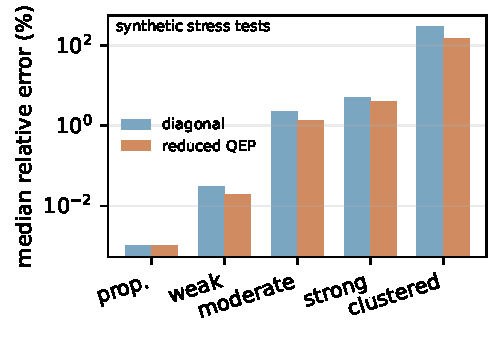
\includegraphics[width=\columnwidth]{figures/fig2_estimator_errors.pdf}
\caption{Synthetic stress-test errors. The diagonal all-mode estimate is excellent in proportional and weak-damping cases, but not robust to strong non-proportional damping or clustered modal frequencies. The reduced QEP is a correction for those regimes, not a replacement for full validation.}
\label{fig:errors}
\end{figure}

This stress test supports the estimator's logic. The contribution is not ``always use the second-order formula'' and not ``the diagonal formula is always enough.'' The contribution is the interpretable correction plus the diagnostic boundary between diagonal-safe, second-order-safe, and QEP-needed regimes.

\subsection{Failure Mechanism of the Diagonal Screen}

The reason for the regime dependence is visible in modal coordinates. Write
\begin{equation}
\Gamma=\Gamma_d+\Gamma_o,
\end{equation}
where $\Gamma_d=\diag(\delta_k)$ and $\Gamma_o$ contains the off-diagonal modal damping. If $\Gamma_o=0$, the QEP decouples. If $\Gamma_o$ is small and modal frequencies are well separated, the pole perturbation induced by off-diagonal damping is small. If two modes are close, however, the same off-diagonal entry can rotate the critical subspace. A scalar estimate based on one unperturbed $q_k$ then misses the actual least-damped combination of modes.

This mechanism explains why a single error number is not enough. A diagonal formula can be nearly exact in weak damping and badly wrong in clustered modes. A reduced QEP can improve clustered cases, but it is not magic: if the selected subspace omits a coupled neighbor, the reduced model still fails. The estimator must therefore report its own diagnostic label, not only a number.

\begin{table}[t]
\centering
\caption{Synthetic stress-test summary. Values are median relative errors against the full first-order eigensolve. The clustered case is intentionally pathological and exposes the failure mechanism.}
\label{tab:synthetic}
\begin{tabular}{lccc}
\toprule
Regime & Diagonal & 2nd order & QEP\\
\midrule
Proportional damping & $\approx 0$ & $\approx 0$ & $\approx 0$\\
Weak heterogeneity & $0.038\%$ & $0.007\%$ & $0.004$--$0.024\%$\\
Moderate heterogeneity & $2.53\%$ & $0.65\%$ & $0.22$--$1.51\%$\\
Strong heterogeneity & $5.16\%$ & $1.46\%$ & $1.24$--$3.90\%$\\
Clustered frequencies & $308\%$ & $74\%$ & $9.8$--$160\%$\\
\bottomrule
\end{tabular}
\end{table}

\subsection{Reduced PLL Check: Network Versus Control}

To test whether the perturbation idea survives beyond the clean second-order surrogate, a reduced seven-state grid-following inverter model was evaluated. The three-node system contains one synchronous generator, one grid-forming inverter, and one grid-following inverter with PLL memory. The state vector is
\begin{equation}
x=[\theta_0,\theta_{\rm pll},\theta_2,\omega_0,\omega_{\rm pll},\omega_2,z_{\rm pll}]^T,
\end{equation}
where $z_{\rm pll}$ is the PLL integral state. The zero-order model sets the PLL memory coupling to zero, so the inverter behaves as a memory-free damping channel. Standard nonsymmetric eigenvalue perturbation then corrects the critical pole of this zero-order matrix.

In the canonical reduced case, the full critical pole is approximately $-0.034236\pm j1.177983$. The zero-order pole is $-0.034827+j1.178430$, and the second-order correction moves it to $-0.034154+j1.177846$, reducing the complex-pole distance from $7.41\times10^{-4}$ to $1.60\times10^{-4}$. Over 399 stable randomized reduced-PLL cases, the median damping-margin error falls from $2.16\%$ at order zero to $0.09\%$ at order two, while the 95th-percentile error falls from $29.2\%$ to $12.9\%$.

This result supports the network-vs-control interpretation: the zero-order margin is the electromechanical network prediction, while the second-order term measures how PLL memory shifts the critical pole. It is not a substitute for ANDES validation. The model is reduced and deliberately transparent; current loops, limiters, algebraic network constraints, and vendor-grade IBR models remain outside this test.

\section{ANDES IEEE 39-Bus Simulations}

\subsection{Baseline Synchronous Case}

The first IEEE 39-bus experiment was run in ANDES 2.0.0 using the packaged \texttt{ieee39\_full.xlsx} case. The case contains 39 buses, 46 lines, 10 GENROU machines, 10 IEEEST/PSS devices, and no active REGCA1, REGCP1, REGF1, REGF2, or PLL1 devices. Thus it is a synchronous-generator benchmark, not a full IBR benchmark. Power flow and eigenanalysis completed. The linearized model has 160 eigenvalues, 64 oscillatory eigenvalues, two zeros, and nine positive-real non-oscillatory modes. The least-damped stable oscillatory pair is
\begin{equation}
s_\star=-1.3460\pm j\,8.6115,\qquad \zeta_\star=0.1544,
\end{equation}
with oscillation frequency $1.3706$ Hz. The positive-real non-oscillatory modes are reported as a case-quality warning; they do not support a final practical stability claim.

\begin{table}[t]
\centering
\caption{ANDES IEEE39 baseline simulation summary.}
\label{tab:andesbaseline}
\begin{tabular}{lc}
\toprule
Quantity & Value\\
\midrule
Buses / lines & 39 / 46\\
Synchronous machines & 10 GENROU\\
IBR dynamic devices & 0 REGCP1/REGF1/PLL1\\
Linearized eigenvalues & 160\\
Oscillatory eigenvalues & 64\\
Positive-real eigenvalues & 9 non-oscillatory\\
Least-damped stable pole & $-1.3460\pm j8.6115$\\
Damping ratio / frequency & $0.1544$ / $1.3706$ Hz\\
\bottomrule
\end{tabular}
\end{table}

\subsection{Positive-Mode Diagnostic}

A participation-factor audit was run to identify the source of those positive-real modes. The dominant positive modes participate primarily in \texttt{TGOV1N}, \texttt{IEEEX1}/\texttt{IEEEST}, and internal \texttt{GENROU} transient-voltage states rather than in electromechanical angle-frequency pairs. A control experiment removed model families from the packaged case. Removing only \texttt{TGOV1N} reduced the count from nine positive modes to four, while removing only \texttt{IEEEST} removed all positive-real modes; the least-damped oscillatory pair remained essentially unchanged at approximately $\zeta=0.1545$ and $1.3705$ Hz. Thus the positive modes appear to be a stabilizer-model artifact in the packaged dynamic case, not a network oscillation claim. The baseline is therefore useful for reproducible extraction tests, but the manuscript should not cite it as evidence of a physically unstable New England benchmark.

\begin{table}[t]
\centering
\caption{ANDES diagnostic simulations for positive-real modes in the packaged IEEE39 dynamic case.}
\label{tab:andesdiagnostic}
\begin{tabular}{lccc}
\toprule
Variant & Removed & Pos. modes & $\zeta_{\rm osc}$\\
\midrule
Base & -- & 9 & 0.1544\\
No governor & TGOV1N & 4 & 0.0568\\
No PSS & IEEEST & 0 & 0.1545\\
No exciter/PSS & IEEEX1, IEEEST & 0 & 0.1538\\
GENROU only & Controls & 0 & 0.0606\\
\bottomrule
\end{tabular}
\end{table}

\subsection{IEEE39-Derived Kron Surrogate}

To exercise the proposed estimator on the IEEE 39 topology before a full IBR dynamic case is built, the solved network was converted into a generator-bus surrogate. The active-power stiffness Laplacian was assembled from the solved line series admittances and bus angles, then Kron-reduced from 39 buses to the 10 generator buses. IBR-like scenarios were generated by reducing effective inertia and introducing heterogeneous local damping at a penetration level $\rho$. The reference for this surrogate test is the full QEP of the Kron-reduced second-order model, not the full ANDES DAE.

\begin{table}[t]
\centering
\caption{IEEE39-derived surrogate estimator errors. Values are relative error against the full QEP of the Kron-reduced surrogate, not full IBR ANDES errors.}
\label{tab:ieee39surrogate}
\begin{tabular}{lccc}
\toprule
Estimator & Median & 95th pct. & Mean\\
\midrule
Diagonal all-mode & $0.468\%$ & $24.15\%$ & $4.18\%$\\
Second order & $0.032\%$ & $9.91\%$ & $1.75\%$\\
Reduced QEP ($r=6$) & $0.037\%$ & $5.44\%$ & $1.09\%$\\
Adaptive & $0.031\%$ & $7.43\%$ & $1.63\%$\\
\bottomrule
\end{tabular}
\end{table}

Table~\ref{tab:ieee39surrogate} supports the same mechanism as the random ensembles: the second-order correction reduces the median error of the diagonal screen by about one order of magnitude, but the reduced QEP has the better tail. The adaptive workflow is therefore still necessary. In the representative $\rho=0.6$ scenario, increasing local damping by 10\% gives the largest margin improvement at generator bus 30 ($\Delta\zeta=0.0112$), followed by buses 38 and 36. For line reinforcements, strengthening line 25--37 gives the largest margin increase ($\Delta\zeta=0.00631$), while strengthening lines 2--3, 25--26, 1--2, 3--4, and 1--39 reduces the damping margin even though the critical modal stiffness increases. Fig.~\ref{fig:ieee39resultmap} overlays these surrogate planning results with the Mix60 replacement map and the Phase-1 ANDES audit status. This is a damping-aware Braess-like reversal in the surrogate, not yet a full ANDES IBR topology claim.

\begin{figure*}[t]
\centering
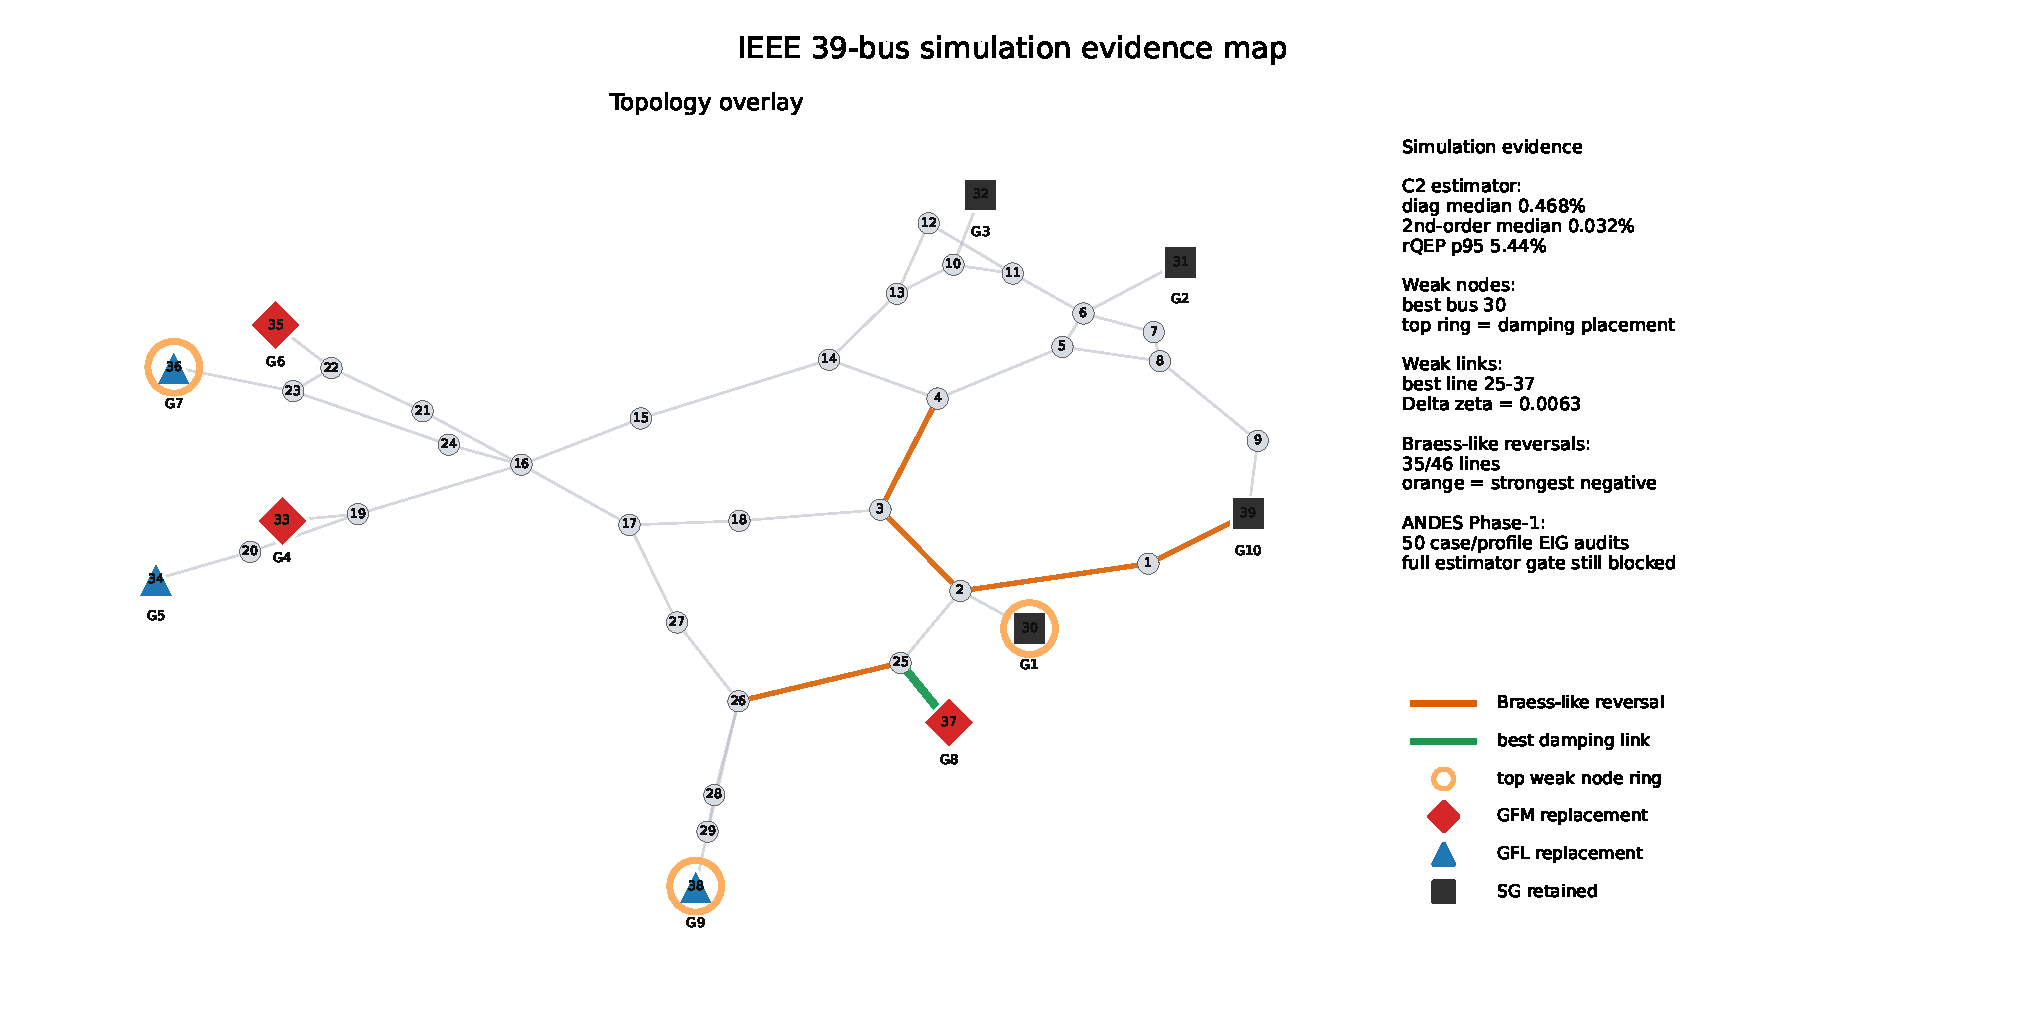
\includegraphics[width=0.96\textwidth]{figures/fig6_ieee39_result_map.pdf}
\caption{IEEE 39-bus evidence map for the current draft. The topology overlay combines the Mix60 SG/GFL/GFM replacement map with IEEE39-derived surrogate results: orange lines are the strongest Braess-like damping reversals, the green line is the best damping-aware reinforcement, and orange rings mark the top weak-node damping-placement buses. The right panel lists the estimator and calibration-audit evidence used in the paper. This figure is a traceability map, not final validation against calibrated full-ANDES IBR poles.}
\label{fig:ieee39resultmap}
\end{figure*}

\subsection{SG-to-GFL/GFM Replacement Cases}

To close the gap between the packaged synchronous benchmark and a true IBR benchmark, a case-generation script was added for direct SG-to-IBR replacement in ANDES. The static \texttt{PV}/\texttt{Slack} devices are retained so that the original power-flow dispatch is preserved. For each converted generator, the associated \texttt{GENROU}, governor, exciter, and PSS rows are removed from the derived case. Grid-following replacements use \texttt{REGCP1}, \texttt{REECA1}, \texttt{REPCA1}, and \texttt{PLL1}; grid-forming replacements use \texttt{REGF1}. The slack generator is kept synchronous in all pilot cases.

\begin{figure*}[t]
\centering
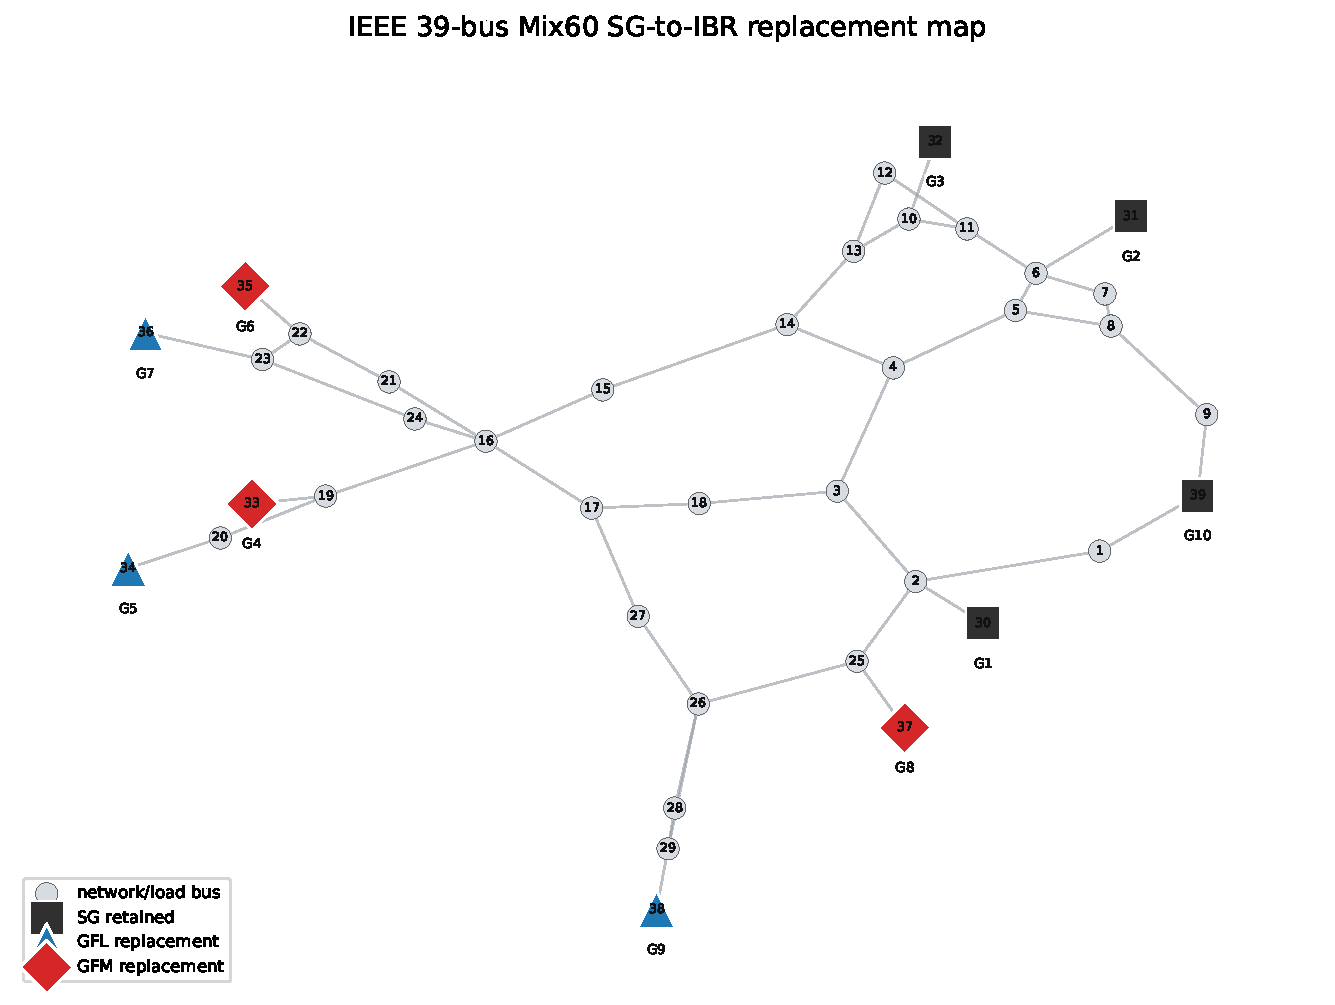
\includegraphics[width=0.93\textwidth]{figures/fig5_ieee39_ibr_map.pdf}
\caption{IEEE 39-bus topology and the Mix60 SG-to-IBR replacement map used in the ANDES pilot. Generators 5, 7, and 9 are replaced by GFL devices at buses 34, 36, and 38; generators 4, 6, and 8 are replaced by GFM devices at buses 33, 35, and 37; generators 1, 2, 3, and 10 remain synchronous at buses 30, 31, 32, and 39. This figure documents the benchmark construction. It is not, by itself, estimator validation.}
\label{fig:ieee39ibrmap}
\end{figure*}

\begin{table*}[t]
\centering
\caption{Full ANDES IEEE39 SG-to-IBR replacement pilot simulations. All cases solved power flow and eigenanalysis. Stability is assessed from the full linearized DAE with generic uncalibrated controller parameters.}
\label{tab:andesibrcases}
\begin{tabular}{lccccccc}
\toprule
Case & GFL gens & GFM gens & GENROU left & Pos. modes & Max $\Real(s)$ & Stable & $\zeta_{\rm osc}$ / Hz\\
\midrule
GFL20 & 9,8 & -- & 8 & 1 & 1.012 & no & 0.1148 / 13.7277\\
GFM20 & -- & 9,8 & 8 & 6 & 4.291 & no & 0.1438 / 1.3910\\
Mix20 & 9 & 8 & 8 & 3 & 1.070 & no & 0.1370 / 13.7507\\
Mix40 & 9,7 & 8,6 & 6 & 2 & 1.072 & no & 0.1266 / 13.7856\\
Mix60 & 9,7,5 & 8,6,4 & 4 & 0 & $2.0{\times}10^{-9}$ & yes & 0.1236 / 13.7417\\
\bottomrule
\end{tabular}
\end{table*}

Table~\ref{tab:andesibrcases} gives the first full-ANDES construction result, and Fig.~\ref{fig:ieee39ibrmap} shows the exact bus-level replacement map for the stable Mix60 pilot. All five derived cases load, solve power flow, and run eigenanalysis. Four low-penetration pilot cases retain positive-real modes under the uncalibrated generic controller parameters; the 60\% mixed GFL/GFM case has no positive-real eigenvalues under the same tolerance. The stable oscillatory damping ratios in the table are therefore not used as final validation of the estimator. Their immediate value is methodological: the workflow can now generate reproducible IEEE39 cases with active \texttt{REGCP1}/\texttt{PLL1} and \texttt{REGF1} dynamics, and the next validation step is to calibrate controller parameters and extract a physically matched reduced surrogate from the full ANDES state matrix.

The frequency column in Table~\ref{tab:andesibrcases} is computed as $|\Imag(s)|/(2\pi)$, so the entries near $13.7$ Hz are not a rad/s-to-Hz unit error. A participation-factor audit shows that these high-frequency least-damped stable modes are dominated by control or auxiliary states, such as \texttt{IEEEST}/\texttt{IEEEX1}, \texttt{REGF1}, \texttt{PLL1}, or \texttt{BusFreq} states, rather than by a low-frequency inter-area electromechanical mode. This is consistent with the central warning of the paper: once IBR and controller states are active, the least-damped stable mode need not be the familiar low-frequency network mode.

\subsection{Controller-Aware Rational Bridge by Contour Integration}

The failed scalar bridge is not a failure of the full ANDES eigensolve; it is a failure of the coefficient model. In the packaged and derived cases, the physical \texttt{GENROU.D} entries are zero, while the observed modal damping is supplied by controller, exciter, governor, stabilizer, PLL, and inverter states. The appropriate reduced object is therefore not a constant-coefficient scalar QEP with a nodal $D$. It is a rational nonlinear eigenvalue problem (NEP) in which the condensed control states enter as a frequency-dependent self-energy.

Partition the full ANDES state matrix as
\begin{equation}
A=\begin{bmatrix}A_{ee} & A_{ec}\\ A_{ce} & A_{cc}\end{bmatrix},
\end{equation}
where $x_e$ contains the retained network/interface states and $x_c$ contains all condensed controller and auxiliary states. In second-order notation the bridge is
\begin{equation}
T(s)=s^2M+s\Sigma(s)+\Lt,\qquad
\Sigma(s)=D_0+C(sI-A_{cc})^{-1}B.
\label{eq:rationalnep}
\end{equation}
The implementation solves the equivalent first-order Schur NEP
\begin{equation}
S_e(s)=sI-A_{ee}-A_{ec}(sI-A_{cc})^{-1}A_{ce},
\label{eq:schurnep}
\end{equation}
which avoids forcing an artificial $M,D_0,\Lt$ factorization when grid-forming angle states and controller states are mixed. When the retained states are clean $\delta$--$\omega$ pairs, \eqref{eq:schurnep} is the first-order form of \eqref{eq:rationalnep}.

Zeros of \eqref{eq:schurnep} were extracted with Beyn contour integration. For a probing matrix $\widehat V$, the moments are
\begin{align}
A_0&=\frac{1}{2\pi j}\oint_\Gamma S_e(s)^{-1}\widehat V\,ds,\\
A_1&=\frac{1}{2\pi j}\oint_\Gamma sS_e(s)^{-1}\widehat V\,ds.
\end{align}
After the SVD of $A_0$, the reduced matrix $U_K^\ast A_1 W_K\Sigma_K^{-1}$ gives the zeros inside $\Gamma$. A local polish was used only after the contour extraction: it starts from each Beyn Ritz value and solves for the minimum-modulus eigenvalue of $S_e(s)$ to vanish. The polish receives no ANDES pole, mode index, frequency, or damping target; ANDES poles are used only after extraction for validation.

Two contours were used. The \emph{network-margin} contour covers $\Real(s)\in[-4,0.8]$ and $\Imag(s)\in[3.5,12]$ rad/s. The \emph{PLL-control} contour covers $\Real(s)\in[-25,0.8]$ and $\Imag(s)\in[60,95]$ rad/s. Completeness was checked with the argument principle,
\begin{equation}
N_\Gamma=\frac{1}{2\pi j}\oint_\Gamma \operatorname{tr}\left(S_e(s)^{-1}S_e'(s)\right)ds,
\label{eq:argumentcount}
\end{equation}
with the count corrected by the number of $A_{cc}$ poles inside the contour. The extracted zero counts agree with \eqref{eq:argumentcount}: for no-PSS and base, the network-margin contour extracts $9$ zeros versus argument counts $9.00006$ and $9.00007$; for Mix60, the network-margin contour extracts $4$ zeros versus $4.00003$, and the PLL-control contour extracts $3$ zeros versus $2.999998$ after adding the three $A_{cc}$ poles inside the contour.

\begin{table*}[t]
\centering
\caption{Phase-0D controller-aware rational bridge validation. NEP-Beyn poles are extracted by contour integration and then compared against the full ANDES eigensolve. Frequency and damping errors are relative percentages.}
\label{tab:phase0d}
\scriptsize
\begin{tabular}{@{}p{0.10\textwidth}p{0.20\textwidth}p{0.20\textwidth}p{0.11\textwidth}p{0.11\textwidth}p{0.16\textwidth}@{}}
\toprule
Case & ANDES critical pole & NEP-Beyn critical pole & Freq. error & Damping error & $\pi_c$ / family\\
\midrule
no-PSS
& $-1.34635+j8.61104$
& $-1.34635+j8.61104$
& $4.86{\times}10^{-14}\%$
& $6.29{\times}10^{-13}\%$
& $0.680$ / I-network\\
base
& $-1.34601+j8.61148$
& $-1.34601+j8.61148$
& $1.62{\times}10^{-13}\%$
& $1.06{\times}10^{-12}\%$
& $0.653$ / I-network\\
Mix60
& $-10.7514+j86.3419$
& $-10.7514+j86.3419$
& $8.47{\times}10^{-11}\%$
& $2.48{\times}10^{-9}\%$
& $0.853$ / II-control\\
\bottomrule
\end{tabular}
\end{table*}

Table~\ref{tab:phase0d} shows that the rational bridge reproduces the full ANDES critical poles in all three diagnostic cases. The important case is Mix60. The least-damped stable pole is not the $1.49$ Hz electromechanical mode found by the fixed-point Schur iteration; it is a $13.7417$ Hz control-family pole with $\zeta=0.12357$. The NEP-Beyn bridge extracts that pole from the PLL-control contour with $\pi_c=0.853$. The nearest condensed-control pole is $-10.5593+j86.246$, at distance $0.215$, and the reconstructed condensed states are led by \texttt{PLL1} angle states. Thus the bridge identifies the mechanism that the scalar bridge and the fixed-point Schur iteration missed: the damping-margin mode can belong to the controller family.

\begin{remark}[Fast-control limit]
The static limit $\Sigma(0)=D_0-CA_{cc}^{-1}B$ is a useful way to recover a constant-coefficient QEP only when $A_{cc}$ is invertible. In the base and Mix60 audits, $sI-A_{cc}$ is singular or severely ill-conditioned at $s=0$, consistent with integral controller states. Therefore $\Sigma(0)$ is not the robust validation object for these cases. The robust check is the contour NEP itself, evaluated against the full ANDES poles at the relevant nonzero critical frequencies.
\end{remark}

\subsection{NEP-Enabled Control-Resonant Reinforcement Reversal}

The validated Schur NEP bridge also makes it possible to distinguish two different reasons why a line reinforcement can reduce damping ratio. The first is the geometric effect already visible in a scalar modal model: reinforcement can increase modal stiffness or frequency without increasing decay enough, so $\zeta=-\Real(s)/|s|$ decreases. The second is a controller-mediated resonant effect: reinforcement can move a network-family mode toward a condensed-control pole, making the frequency-dependent self-energy dominate the pole sensitivity. The second mechanism is invisible to a scalar $(L,M,D)$ bridge because it depends on the resolvent $(sI-A_{cc})^{-1}$.

For a line parameter $w$, the Schur-NEP pole sensitivity is
\begin{align}
\frac{ds}{dw}
&=-\frac{y^\ast(\partial S_e(s)/\partial w)x}
{y^\ast S_e'(s)x}, \nonumber\\
S_e'(s)
&=I+A_{ec}(sI-A_{cc})^{-2}A_{ce}.
\label{eq:schursens}
\end{align}
where $x$ and $y$ are right and left null vectors of $S_e(s)$. In the audit below, the numerator is decomposed into three diagnostic parts: (A) a retained stiffness/frequency contribution from the retained $\omega$--$\delta$ block, (B) a retained-network residual that includes modal rotation within the retained coordinates, and (C) the condensed-control self-energy contribution. A reversal is called \emph{resonant} only if the network-family damping decreases, the tracked mode moves closer to a matched $A_{cc}$ pole, the nearest condensed-control pole is PLL-dominated, and the negative C term dominates the A and B terms.

\begin{table*}[t]
\centering
\caption{NEP-enabled control-resonant reinforcement audit. The example is the largest global-margin resonant reversal found under a 1\% line-strengthening perturbation. The result is a modal-local mechanism: the affected network mode is not the global damping-margin pole in this benchmark.}
\label{tab:resonantbraess}
\scriptsize
\begin{tabular}{@{}p{0.25\textwidth}p{0.20\textwidth}p{0.22\textwidth}p{0.22\textwidth}@{}}
\toprule
Quantity & Mix60/no-PSS Line 44 & Soft-GFL negative control & Interpretation\\
\midrule
Line and buses & Line 44, 23--36 & Same line and mode rank & Same physical reinforcement test.\\
Global margin change & $\Delta\zeta_{\min}=-2.750{\times}10^{-5}$ & $\Delta\zeta_{\min}=+2.0{\times}10^{-6}$ & The resonant case slightly lowers the system margin; the negative control does not.\\
Network-mode change & $\Delta\zeta_{\rm net}=-3.581{\times}10^{-5}$ & $\Delta\zeta_{\rm net}=+4.6{\times}10^{-5}$ & The mechanism acts on a network-family secondary mode.\\
Distance to matched $A_{cc}$ pole & $3.332\rightarrow3.330$ & $8.200\rightarrow8.199$ & The resonant case is close to a condensed-control pole; soft-GFL moves the pole away.\\
Relative distance & $0.0368$ & $0.9167$ & Control proximity is about $25\times$ smaller in the resonant case.\\
Control denominator fraction & $0.959$ & $0.0789$ & The resonant case is dominated by frequency-dependent control self-energy.\\
Dominant condensed states & \texttt{PLL1} G9/G5/G7 & Not PLL-dominated & The observed resonance is PLL-related.\\
A stiffness term & $-1.1{\times}10^{-9}$ & $-2.98{\times}10^{-4}$ & Geometric stiffness is not the resonant driver.\\
B retained-rotation term & $\approx0$ & $-5.4{\times}10^{-5}$ & Retained-network rotation is also not dominant.\\
C self-energy term & $-3.583{\times}10^{-3}$ & $+4.927{\times}10^{-3}$ & The self-energy term sets the sign and disappears as a reversal under soft-GFL.\\
\bottomrule
\end{tabular}
\end{table*}

\begin{figure}[t]
\centering
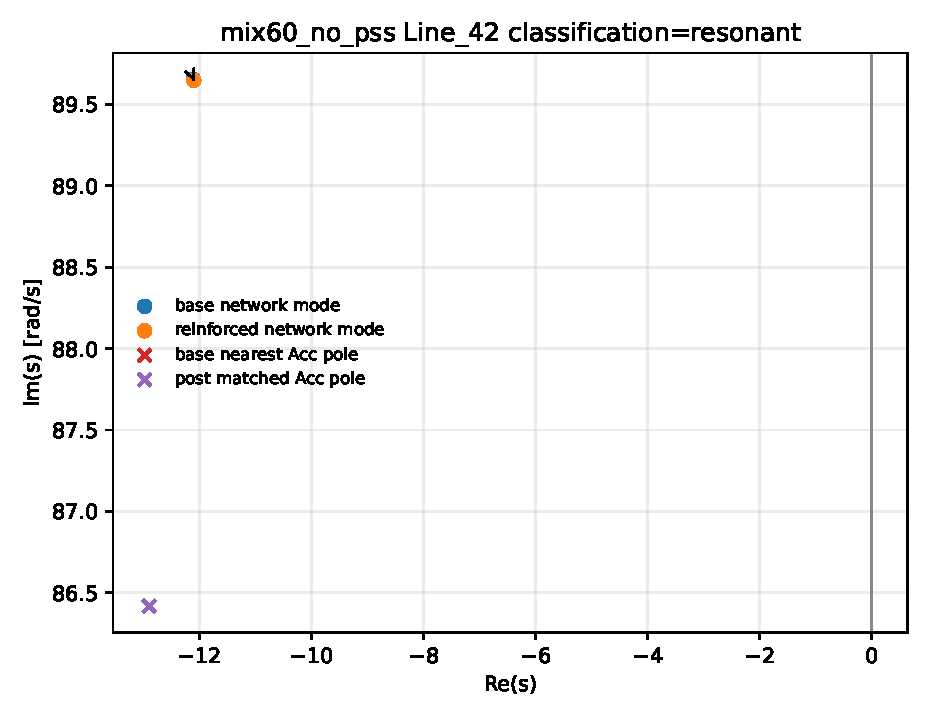
\includegraphics[width=\columnwidth]{figures/fig7_braess_nep_s_plane.pdf}
\caption{Control-resonant reinforcement audit in the Schur-NEP plane. The validated NEP bridge tracks a network-family mode and nearby condensed-control poles. In the resonant case, strengthening Line 44 moves the network mode toward a PLL-dominated $A_{cc}$ pole and the self-energy term dominates the damping decrease.}
\label{fig:resonantbraess}
\end{figure}

Across Mix60, Mix60/no-PSS, and Mix60/soft-GFL audits, 348 line/mode records reduce the global margin and 232 reduce a tracked network-family mode. Forty records satisfy the strict resonant criteria above. All 40 have $|C|>10\max(|A|,|B|)$; the median dominance ratio is $1039\times$, so these cases are not geometric reversals mislabeled as resonant. The largest global effect in Table~\ref{tab:resonantbraess} remains small in absolute magnitude, and none of the 40 resonant cases makes the resonant network mode the global critical pole. The global margin remains set by a control-family pole in every resonant row. The claim is therefore deliberately limited: the bridge confirms a genuine, control-conditional, modal-local resonant mechanism, not a universal or dominant cause of margin collapse.

The soft-GFL control profile is the required negative control. For the same line/mode pairs that are resonant in Mix60/no-PSS, the median relative distance from the network mode to the nearest condensed-control pole increases from $0.0368$ to $0.9167$, while the denominator fraction associated with the frequency-dependent control term falls from $0.959$ to $0.0789$. Thus the mechanism turns off when the spectral condition predicted by the theory is removed. This distinction is actionable. A geometric reinforcement reversal is mitigated by changing modal damping or accepting the frequency--damping tradeoff; a resonant network-control reversal requires retuning the control pole or avoiding the reinforcement that pulls the network mode into that pole.

\subsection{Hidden Control-Resonance Margin}

The same NEP geometry gives a warning metric that is not visible in a static scalar bridge. A system may have all poles in the left half-plane and an acceptable present damping ratio, while a network-family mode lies close to a condensed-control pole. In that case, a small admissible topology or control perturbation can move the network-family mode into a frequency region where the resolvent $(sI-A_{cc})^{-1}$ and the derivative term $(sI-A_{cc})^{-2}$ dominate the pole sensitivity.

For a NEP zero $s_k$ and condensed-control pole $\mu_j\in\operatorname{spec}(A_{cc})$, define the normalized control-pole distance
\begin{equation}
d_{kj}^{\rm ctrl}=
\frac{|s_k-\mu_j|}{|s_k|+|\mu_j|}.
\label{eq:hiddencontroldistance}
\end{equation}
Let
\begin{equation}
\phi_k^{\Sigma}=
\frac{\left|y_k^\ast s_k\Sigma'(s_k)x_k\right|}
{\left|y_k^\ast T_s(s_k)x_k\right|+\epsilon},
\label{eq:selfenergyfraction}
\end{equation}
where $x_k$ and $y_k$ are right and left null vectors of $T(s_k)$ and $\epsilon$ is a small numerical regularizer. A small $d_{kj}^{\rm ctrl}$ together with large $\phi_k^\Sigma$ indicates a hidden control-resonance margin: the present pole may look safe, but its sensitivity is already governed by nearby control dynamics.

The reason this metric is not visible in a constant-coefficient bridge is the resolvent bound. Let
\begin{equation}
\Delta_c(s)=\operatorname{dist}\!\left(s,\operatorname{spec}(A_{cc})\right).
\end{equation}
If $A_{cc}$ is diagonalizable with eigenvector condition number $\kappa_c$, then for $s\notin\operatorname{spec}(A_{cc})$,
\begin{align}
\norm{(sI-A_{cc})^{-1}}
&\le \frac{\kappa_c}{\Delta_c(s)},\nonumber\\
\norm{\Sigma'(s)}
&\le
\frac{\norm{C}\norm{B}\kappa_c^2}{\Delta_c(s)^2}.
\label{eq:resolventbound}
\end{align}
Thus a pole may have acceptable $\zeta_k$ while its sensitivity denominator is dominated by $s\Sigma'(s_k)$ because the distance $\Delta_c(s_k)$ is small. This is the proposed \emph{hidden} margin: it is a distance-to-control-resonance margin, not only a present damping-ratio margin.

For any admissible action parameter $p$, the exact local NEP sensitivity is
\begin{align}
\frac{\partial s_k}{\partial p}
&=
-\frac{y_k^\ast T_p(s_k)x_k}
{y_k^\ast T_s(s_k)x_k},
\label{eq:genericnepsens}\\
T_s(s)
&=2sM+\Sigma(s)+s\Sigma'(s),
\nonumber\\
T_p(s)
&=s^2M_p+s\Sigma_p(s)+L_p .
\nonumber
\end{align}
The induced damping-ratio derivative is
\begin{equation}
\frac{\partial\zeta_k}{\partial p}
=-\frac{\Real(s_{k,p})}{|s_k|}
\frac{\Real(s_k)\Real(\overline{s_k}s_{k,p})}{|s_k|^3},
\qquad
s_{k,p}=\frac{\partial s_k}{\partial p}.
\label{eq:zetanepsens}
\end{equation}
Equations \eqref{eq:genericnepsens}--\eqref{eq:zetanepsens} define a common sensitivity language for line, inertia, shunt, damping, and controller actions.

For a target damping ratio $\zeta_\star$, define the first-order damping action margin
\begin{equation}
m_p^{\zeta}(k)=
\frac{\zeta_k-\zeta_\star}
{\left[-\partial\zeta_k/\partial p\right]_+},
\qquad [a]_+=\max(a,0),
\label{eq:hiddenactionmargin}
\end{equation}
with $m_p^{\zeta}=\infty$ when the action does not decrease damping to first order. For a minimum allowed control-pole distance $d_\star$, define the resonance-distance action margin
\begin{equation}
m_p^{d}(k,j)=
\frac{d_{kj}^{\rm ctrl}-d_\star}
{\left[-\partial d_{kj}^{\rm ctrl}/\partial p\right]_+}.
\label{eq:distancemargin}
\end{equation}
The combined hidden safety margin is then
\begin{equation}
m_p^{\rm hid}(k,j)
=\min\{m_p^{\zeta}(k),m_p^{d}(k,j)\},
\label{eq:combinedhiddenmargin}
\end{equation}
and the system-level margin over an action set $\mathcal{P}$ is
\begin{equation}
m_{\mathcal{P}}^{\rm hid}
=\min_{k\in\mathcal{K}}\min_{j}\min_{p\in\mathcal{P}}
m_p^{\rm hid}(k,j),
\label{eq:hiddenmargin}
\end{equation}
restricted to tracked oscillatory network-family modes $\mathcal{K}$ or to all oscillatory zeros, depending on the claim. This is not a collapse certificate. It is a local damping-resonance vulnerability metric: it asks how much admissible topology or control movement is needed before a currently acceptable pole crosses the target damping margin.

This definition also gives controller-aware weak elements. A weak node is not defined by graph centrality alone, but by local pole movement through the rational self-energy. For a node action set $\mathcal{P}_i$,
\begin{equation}
\mathcal{W}_i^{\rm hid}
=
\max_{k,j}\max_{p\in\mathcal{P}_i}
\phi_k^\Sigma
\left[-\frac{\partial\zeta_k}{\partial p}\right]_+
\left[-\frac{\partial d_{kj}^{\rm ctrl}}{\partial p}\right]_+ .
\label{eq:resolventweaknode}
\end{equation}
A large $\mathcal{W}_i^{\rm hid}$ means that an admissible local action both reduces damping and pulls a pole toward a condensed-control resonance. The scalar sensitivities remain useful diagnostics,
\begin{equation}
W_i^{D}=-\frac{\partial\zeta_c}{\partial D_i},\quad
W_i^{M}=-\frac{\partial\zeta_c}{\partial M_i},\quad
W_i^{\kappa}=-\frac{\partial\zeta_c}{\partial \kappa_i},
\label{eq:weaknode}
\end{equation}
where $\kappa_i$ denotes a local controller parameter such as PLL gain, droop, or virtual-inertia tuning. A weak link is analogously
\begin{equation}
W_e=-\frac{\partial\zeta_c}{\partial w_e}.
\label{eq:weaklink}
\end{equation}
The sign matters: $W_e>0$ means strengthening that link lowers damping to first order. A resolvent-aware weak link uses the same hidden score,
\begin{equation}
\mathcal{W}_e^{\rm hid}
=
\max_{k,j}
\phi_k^\Sigma
\left[-\frac{\partial\zeta_k}{\partial w_e}\right]_+
\left[-\frac{\partial d_{kj}^{\rm ctrl}}{\partial w_e}\right]_+ .
\label{eq:resolventweaklink}
\end{equation}
A \emph{hidden-resonant} weak link has $\mathcal{W}_e^{\rm hid}>0$ for a matched control pole. Thus the graph object being ranked is no longer only a line in $L$; it is a line whose perturbation moves a pole through the rational self-energy geometry.

\subsection{Instability-Flow Weak Nodes and Links}

The previous definitions rank weak elements by local margin loss. The same NEP sensitivity can be expanded into an instability-flow interpretation: a disturbance enters through a physical node or line, excites retained network modes, couples through the rational self-energy to condensed control poles, and then moves the damping margin. This subsection derives that object step by step.

Assume first that $A_{cc}$ is diagonalizable. Let
\begin{equation}
A_{cc}v_p=\mu_pv_p,\qquad
w_p^\ast A_{cc}=\mu_pw_p^\ast,\qquad
w_p^\ast v_q=\delta_{pq}.
\end{equation}
Then
\begin{equation}
(sI-A_{cc})^{-1}
=\sum_p\frac{v_pw_p^\ast}{s-\mu_p},
\label{eq:controlresolventexpansion}
\end{equation}
and
\begin{equation}
\Sigma(s)
=D_0+\sum_p
\frac{Cv_pw_p^\ast B}{s-\mu_p}.
\label{eq:selfenergycontrolpoleexpansion}
\end{equation}
A retained-network pole $s_k$ is therefore exposed to a condensed-control pole $\mu_p$ only when the poles are close and the input/output projections through $B$ and $C$ are nonzero. A sensitivity-weighted resonance score is
\begin{equation}
R_{kp}^{\rm ctrl}
=
\frac{
|y_k^\ast C v_p|\,|w_p^\ast Bx_k|
}{
|s_k-\mu_p|^2+\epsilon
}.
\label{eq:modalcontrolresonanceweight}
\end{equation}
The squared distance is used because $\Sigma'(s)$ contains $(s-\mu_p)^{-2}$; \eqref{eq:modalcontrolresonanceweight} is a pole-sensitivity weight, not only a distance score.

For a line $e=(i,j)$ with incidence vector $b_e=e_i-e_j$, let $G_e=b_eb_e^T$ denote the normalized stiffness direction. If a line perturbation also changes the operating point or controller condensation, the full local pole sensitivity is
\begin{equation}
\frac{\partial s_k}{\partial w_e}
=
-
\frac{
y_k^\ast\left(G_e+s_k\Sigma_{w_e}(s_k)\right)x_k
}{
y_k^\ast T_s(s_k)x_k
}.
\label{eq:linesenspolefull}
\end{equation}
In a frozen-controller network screen, $\Sigma_{w_e}=0$. In a symmetric graph-modal approximation with $x_k=y_k=q_k$,
\begin{equation}
q_k^TG_eq_k=(b_e^Tq_k)^2,
\label{eq:linegraphfourierparticipation}
\end{equation}
so the graph-Fourier line participation in mode $k$ is
\begin{equation}
\chi_{e,k}=|b_e^Tq_k|^2.
\label{eq:lineparticipation}
\end{equation}
For the full NEP, the analogous normalized participation is
\begin{equation}
\chi_{e,k}^{\rm NEP}
=
\frac{|y_k^\ast G_ex_k|}
{\norm{y_k}\norm{G_e}\norm{x_k}+\epsilon}.
\label{eq:lineparticipationnep}
\end{equation}

Equation~\eqref{eq:linegraphfourierparticipation} also explains modal propagation. For two graph modes $q_k$ and $q_\ell$,
\begin{equation}
q_k^TG_eq_\ell=(b_e^Tq_k)(b_e^Tq_\ell).
\label{eq:linecrossmodal}
\end{equation}
Thus a line is not weak merely because it has high active-power loading. It is weak when it couples the active mode to nearby network modes or to control-pole resonances that reduce damping. A line-level instability current is
\begin{equation}
I_e^{\rm inst}
=
\sum_{k,p}
\chi_{e,k}^{\rm NEP}
R_{kp}^{\rm ctrl}
\left[-\frac{\partial\zeta_k}{\partial w_e}\right]_+ .
\label{eq:lineinstabilitycurrent}
\end{equation}
The three factors have distinct roles: $\chi_{e,k}^{\rm NEP}$ says the line moves the retained mode, $R_{kp}^{\rm ctrl}$ says the mode is exposed to a condensed-control pole, and the final factor keeps only line actions that lower damping to first order.

The associated modal resonance graph is
\begin{equation}
\mathcal{G}_{\rm res}
=
\left(\mathcal{V}_{\rm net}\cup\mathcal{V}_{\rm ctrl},
\mathcal{E}_{\rm res}\right),
\quad
\mathcal{V}_{\rm net}=\{s_k\},\ 
\mathcal{V}_{\rm ctrl}=\{\mu_p\},
\label{eq:modalresonancegraph}
\end{equation}
with edge weights $R_{kp}^{\rm ctrl}$. This is not the bus graph. It is a mode--control graph that identifies which network-family poles are dynamically close to controller-family poles.

The same construction gives node scores. In a graph-modal approximation, node $i$ participates in mode $k$ through $|q_{k,i}|^2$. A resonance-exposure score is
\begin{equation}
I_i^{\rm res}
=
\sum_{k,p}|q_{k,i}|^2R_{kp}^{\rm ctrl}.
\label{eq:noderesonanceexposure}
\end{equation}
For planning, exposure alone is not enough; an intervention must move a margin. With a local action set $\mathcal{A}_i$, define vulnerability and repairability as
\begin{align}
V_i
&=
\max_{a\in\mathcal{A}_i}
\left[-\frac{\partial m_H}{\partial a}\right]_+,
\label{eq:nodevulnerability}\\
R_i^{\rm repair}
&=
\max_{a\in\mathcal{A}_i}
\frac{\left[\partial m_H/\partial a\right]_+}
{\operatorname{cost}(a)+\epsilon}.
\label{eq:noderepairability}
\end{align}
The distinction is operational. A node can be a strong source of vulnerability while still being a poor repair location under cost or actuator limits.

\begin{proposition}[Local weak-element certificate]
\label{prop:localweakelement}
Let $m_H(a)$ be differentiable at the current operating point for a tracked active pole, line, or control-pole pair. If an admissible action $a$ satisfies $\partial m_H/\partial a<0$, then there exists $\bar\epsilon>0$ such that, for all $0<\eta<\bar\epsilon$,
\begin{equation}
m_H(a+\eta)<m_H(a).
\end{equation}
\end{proposition}
\noindent\emph{Proof.}
Taylor expansion gives
\begin{equation}
m_H(a+\eta)
=m_H(a)+\eta\frac{\partial m_H}{\partial a}+o(\eta).
\end{equation}
Because $\partial m_H/\partial a<0$, the first-order term is negative. By the definition of $o(\eta)$, the remainder is smaller in magnitude than half of the negative first-order term for sufficiently small positive $\eta$. Hence $m_H(a+\eta)<m_H(a)$. \hfill$\square$

Proposition~\ref{prop:localweakelement} is intentionally local. It proves that the proposed weak-node and weak-link scores are first-order margin-loss diagnostics. It does not prove that $I_e^{\rm inst}$ or $V_i$ will outperform power-flow loading, betweenness, Fiedler participation, SCR, impedance, or damping-participation rankings in every grid. That is an empirical claim and must be tested against the full NEP or full ANDES eigensolve.

\subsection{Protected-Resolvent Graph-Filter Shaping}

The damping margin is a pole metric. A complementary view is needed when the question is not only where the least-damped pole is, but where a protected input can be amplified into a protected output. This gives an input--output graph-filter certificate. It is especially relevant in non-normal IBR models, where the forcing location and the response location can be spatially separated.

Let
\begin{equation}
G(j\omega)=C_o(j\omega I-A_{\rm sys})^{-1}B_i
\label{eq:protectedresolvent}
\end{equation}
be a protected transfer matrix from disturbance channels $B_i$ to monitored outputs $C_o$. Define the local protected gain
\begin{equation}
g_{\rm prot}=\sigma_1(G(j\omega^\star)),
\qquad
\mathcal{S}_g=\log g_{\rm prot},
\label{eq:protectedgain}
\end{equation}
where $\omega^\star$ is a simple local peak and $\sigma_1$ is simple. Let $u^\star$ and $v^\star$ be the corresponding left and right singular vectors. The two spatial fields
\begin{align}
\phi^{\rm in}
&=(j\omega^\star I-A_{\rm sys})^{-1}B_i v^\star,
\label{eq:phiin}\\
\phi^{\rm out}
&=(j\omega^\star I-A_{\rm sys})^{-H}C_o^H u^\star
\label{eq:phiout}
\end{align}
are the input-forcing and output-response profiles. They are equal only in special normal or nearly collocated cases. Their mismatch is the spatial decoupling that ordinary graph centrality does not see.

\begin{theorem}[Bi-orthogonal protected-resolvent sensitivity]
\label{thm:protectedresolvent}
Assume $\omega^\star$ and $\sigma_1(G(j\omega^\star))$ are locally simple and fixed to first order. For any real parameter $p$ entering only through $A_{\rm sys}$,
\begin{equation}
\boxed{
\frac{\partial \mathcal{S}_g}{\partial p}
=
\frac{1}{g_{\rm prot}}
\Real\!\left[
(\phi^{\rm out})^H
\frac{\partial A_{\rm sys}}{\partial p}
\phi^{\rm in}
\right].}
\label{eq:protectedsens}
\end{equation}
\end{theorem}
\noindent\emph{Proof.}
Let $R=(j\omega^\star I-A_{\rm sys})^{-1}$. Since $dR=R(dA_{\rm sys})R$, the first variation of $G=C_oRB_i$ is
\begin{equation}
dG=C_oR(dA_{\rm sys})RB_i .
\end{equation}
For a simple singular value, $dg_{\rm prot}=\Real[(u^\star)^H(dG)v^\star]$. Substituting the definitions of $\phi^{\rm in}$ and $\phi^{\rm out}$ gives
\begin{equation}
dg_{\rm prot}
=
\Real[(\phi^{\rm out})^H(dA_{\rm sys})\phi^{\rm in}].
\end{equation}
Dividing by $g_{\rm prot}$ gives the derivative of $\log g_{\rm prot}$. \hfill$\square$

The theorem supplies a common exchange rate for topology, damping, inertia, and controller tuning. It is not a substitute for the damping-ratio NEP sensitivity in \eqref{eq:genericnepsens}; it answers a different question. The pole metric asks which action moves the critical pole. The protected-resolvent metric asks which action reduces the worst input--output amplification near the protected frequency band.

For local damping in a second-order state ordering $x=[\theta^T,\omega^T]^T$, the damping perturbation has the velocity block
\begin{equation}
\frac{\partial A_{\rm sys}}{\partial D_i}
=
-\frac{1}{M_i}E_{\omega_i\omega_i},
\end{equation}
so \eqref{eq:protectedsens} gives
\begin{equation}
\boxed{
\frac{\partial \mathcal{S}_g}{\partial D_i}
=
-\frac{1}{g_{\rm prot}M_i}
\Real\!\left[
\overline{\phi^{\rm out}_{\omega_i}}
\phi^{\rm in}_{\omega_i}
\right].}
\label{eq:protectedDsens}
\end{equation}
This is the corrected spatial-decoupling rule. The tempting simplification $-|\phi_i^{\rm out}|^2$ is valid only when input and output fields align. In a non-normal IBR grid, optimal damping placement may follow the bi-orthogonal product, not local inertia deficit or output magnitude alone.

For a line $e=(i,j)$ with incidence vector $b_e=e_i-e_j$, a swing block has
\begin{equation}
\frac{\partial A_{\rm sys}}{\partial w_e}
=
\begin{bmatrix}
0&0\\
-M^{-1}b_eb_e^T&0
\end{bmatrix}
\end{equation}
in the retained network coordinates. Therefore
\begin{equation}
\boxed{
\frac{\partial \mathcal{S}_g}{\partial w_e}
=
-\frac{1}{g_{\rm prot}}
\Real\!\left[
(\phi_{\omega}^{\rm out})^H
M^{-1}b_eb_e^T\phi_{\theta}^{\rm in}
\right].}
\label{eq:protectedlinesens}
\end{equation}
Equation~\eqref{eq:protectedlinesens} is a graph-filter weak-link score: it weights a line by the way it couples the protected forcing profile to the protected response profile. It is not the same as a Fiedler score, a power-flow loading score, or the pole-damping score $W_e$ in \eqref{eq:weaklink}.

\begin{remark}[Relation to weak nodes and weak links]
The weak-element scores now form a hierarchy. The pole score $W_e$ asks whether strengthening line $e$ lowers the damping ratio of a tracked pole. The hidden score $\mathcal{W}_e^{\rm hid}$ asks whether the line also moves that pole toward a condensed-control resonance. The protected-resolvent score \eqref{eq:protectedlinesens} asks whether the same line worsens protected input--output amplification. A robust planning claim should report which of these three certificates is active.
\end{remark}

\begin{theorem}[Flow-feasible dynamic Braess certificate]
\label{thm:flowbraess}
For an operating point with feasible base flows, a line reinforcement direction $w_e$ is a first-order flow-feasible dynamic Braess candidate for the protected resolvent if
\begin{align}
\frac{\partial \nu_c}{\partial w_e}&>0,
\label{eq:braessfreqcond}\\
\frac{\partial \mathcal{S}_g}{\partial w_e}&>0,
\label{eq:braessgaincond}\\
|f_0+\eta J_{f,e}|&\le \bar f
\quad\text{for some }0<\eta\le\bar\eta .
\label{eq:braessflowcond}
\end{align}
Then, for sufficiently small feasible $\eta>0$, the reinforcement improves the stiffness proxy while increasing the protected amplification.
\end{theorem}
\noindent\emph{Proof.}
By differentiability,
\begin{align}
\nu_c(w_e+\eta)&=\nu_c(w_e)+\eta\,\partial\nu_c/\partial w_e+o(\eta),\\
\mathcal{S}_g(w_e+\eta)&=\mathcal{S}_g(w_e)+\eta\,\partial\mathcal{S}_g/\partial w_e+o(\eta).
\end{align}
The signs in \eqref{eq:braessfreqcond}--\eqref{eq:braessgaincond} make the first-order changes positive for sufficiently small $\eta$. Condition \eqref{eq:braessflowcond} restricts the same perturbation to remain within the linearized flow limit. \hfill$\square$

The theorem deliberately uses ``candidate.'' It certifies a local conflict between a stiffness proxy and a protected dynamic certificate under a flow-feasible perturbation. It does not prove that the nonlinear AC dispatch remains feasible for a large switching action, nor that the damping-ratio margin must collapse.

The corresponding local retrofit problem is
\begin{align}
\min_z\quad & c^Tz
\nonumber\\
\text{s.t.}\quad
& \mathcal{S}_{g,0}+\nabla\mathcal{S}_g^Tz\le \mathcal{S}_{g,\star},
\nonumber\\
& F_0+J_Fz\le \bar F,
\nonumber\\
& z_{\min}\le z\le z_{\max},
\label{eq:flowfeasibleretrofit}
\end{align}
where $z=(\Delta w,\Delta D,\Delta M,\Delta\kappa)$ collects topology, damping, inertia, and controller-retuning actions. Equation~\eqref{eq:flowfeasibleretrofit} is a local screening LP; the selected package must be revalidated by the NEP or the full ANDES eigensolve because the active singular vector, active pole, or active flow constraint can switch.

\begin{algorithm}[t]
\caption{Flow-Feasible Protected-Resolvent Retrofitting}
\label{alg:protectedretrofit}
\begin{algorithmic}[1]
\REQUIRE $A_{\rm sys}$, protected channels $B_i,C_o$, action set $\mathcal{A}$, flow limits $\bar F$, costs $c$.
\STATE Compute a local peak $\omega^\star$ and $g_{\rm prot}=\sigma_1(G(j\omega^\star))$.
\STATE Extract singular vectors $u^\star,v^\star$ and fields $\phi^{\rm in},\phi^{\rm out}$ from \eqref{eq:phiin}--\eqref{eq:phiout}.
\STATE For each bus action, compute \eqref{eq:protectedDsens} and the analogous inertia/controller derivatives.
\STATE For each line, compute \eqref{eq:protectedlinesens} and the flow sensitivity $J_{f,e}$.
\STATE Solve the local retrofit LP \eqref{eq:flowfeasibleretrofit}.
\STATE Recompute the NEP or full ANDES eigensolve for the selected package.
\STATE If the active peak, pole family, or flow constraint switches, rebuild the local model and repeat.
\end{algorithmic}
\end{algorithm}

\begin{table*}[t]
\centering
\caption{Status of the protected-resolvent/flow-feasible extension.}
\label{tab:protectedstatus}
\scriptsize
\begin{tabular}{@{}p{0.20\textwidth}p{0.31\textwidth}p{0.21\textwidth}p{0.18\textwidth}@{}}
\toprule
Component & Mathematical status & Current evidence & Claim level\\
\midrule
Bi-orthogonal sensitivity \eqref{eq:protectedsens}
& Direct consequence of singular-value perturbation of the resolvent.
& Implemented in reduced-model coordination gates.
& Valid formula; not new perturbation theory.\\
Spatial decoupling
& General rule is a left--right product, not $-|\phi_i|^2$.
& Gamma gate shows $S_\zeta$ and $S_g$ rankings agree only $21$--$29\%$ for physical profiles.
& Supported phenomenon; mechanism still open.\\
Coordinated packages
& Local LP combines topology, damping, inertia, and controller actions.
& Reduced-model gate: $w+D$ improves over the best single lever in $72.1$--$73.8\%$ across physical Gamma profiles; $w+M$ in $67.2$--$73.8\%$; $D+M$ not robust.
& Reduced-model planning candidate.\\
Nonlinear synergy
& Would require a positive interaction beyond additive first-order value.
& Gate found no robust nonlinear synergy: SynNorm never exceeds the registered $50\%$ threshold.
& Killed as headline.\\
Flow-feasible dynamic Braess
& Theorem~\ref{thm:flowbraess} gives local first-order certificate with flow constraint.
& Needs explicit flow-feasibility runs on calibrated ANDES or DC/AC dispatch sensitivities.
& Proposed next validation.\\
\bottomrule
\end{tabular}
\end{table*}

\begin{table*}[t]
\centering
\caption{Phase-0 validation gates for the full ANDES IEEE39 IBR benchmark.}
\label{tab:phase0gates}
\begin{tabular}{p{0.27\textwidth}p{0.14\textwidth}p{0.52\textwidth}}
\toprule
Gate & Status & Evidence and required next step\\
\midrule
Baseline ANDES load/PFlow/EIG & pass & 39 buses, 46 lines, and 160 eigenvalues; synchronous extraction benchmark only.\\
Positive-mode diagnostic & pass-diagnostic & Removing \texttt{IEEEST}/PSS removes all positive-real modes; report as case-quality warning.\\
SG-to-GFL/GFM case generation & pass & Five derived cases solved power flow and eigenanalysis.\\
Generic IBR small-signal stability & partial & One of five cases is stable under generic gains; controller calibration is still required.\\
Controller-aware rational NEP bridge (contour-validated) & pass & Replaces the failed scalar $(L,M,D)$ bridge. Beyn contour integration reproduces full ANDES critical poles in no-PSS, base, and Mix60; Mix60's 13.7 Hz PLL-family critical mode is captured.\\
Estimator and planning validation vs. full ANDES IBR poles & pending & The bridge is now validated and a resonant line-reinforcement mechanism audit has been completed. Experiments A--E must still compare the diagonal, second-order, reduced-QEP, conversion-ranking, and planning claims against full ANDES poles.\\
\bottomrule
\end{tabular}
\end{table*}

The scripts store the Mix60 topology diagram and supporting JSON/CSV artifacts under \texttt{outputs/ieee39\_phase0\_bridge}, the negative scalar bridge audit under \texttt{outputs/phase0\_physical\_bridge}, the contour-validated NEP audit under \texttt{outputs/phase0d\_nep\_contour\_solver}, and the control-resonant reinforcement audit under \texttt{outputs/phase\_braess\_nep}. The negative scalar audit remains important: it shows why a nodal $D$ extracted from \texttt{GENROU.D} cannot represent full ANDES damping. The Phase-0D result closes the next bridge gap by retaining controller states through the rational self-energy. It does not close the estimator-validation gap: the second-order correction and planning rankings still need registered comparison against full ANDES poles.

\subsection{Phase-1 Controller Calibration Audit}

A first calibration audit was then run on the five derived IBR cases. Ten documented profiles were tested: the original generic parameters; slower PLL gains; softened GFL voltage/reactive controls; softened GFM controls; combined soft profiles; and diagnostic variants that remove retained synchronous-machine \texttt{IEEEST}/PSS or \texttt{IEEEX1}+\texttt{IEEEST} rows. Each profile was evaluated by full ANDES power flow and eigenanalysis, with participation factors recorded for the dominant positive mode and the least-damped stable oscillatory mode.

\begin{table*}[t]
\centering
\caption{Phase-1 controller calibration audit. Diagnostic profiles remove retained synchronous-machine controls and are not final tuning recommendations.}
\label{tab:phase1calibration}
\scriptsize
\begin{tabular}{@{}p{0.12\textwidth}p{0.25\textwidth}p{0.25\textwidth}p{0.29\textwidth}@{}}
\toprule
Case & Best controller-only profile & Best diagnostic profile & Mode audit\\
\midrule
GFL20
& Very-soft IBR controls: 1 positive mode, max $\Real(s)=1.011$.
& No PSS plus soft IBR controls: stable, max $\Real(s)=4.0{\times}10^{-10}$.
& Generic positive mode dominated by \texttt{REECA1}; high-frequency stable modes are control/auxiliary dominated.\\
GFM20
& Baseline remains best: 6 positive modes, max $\Real(s)=4.291$.
& No exciter/PSS: still 2 positive modes, max $\Real(s)=4.286$.
& Remaining instability is not cleared by tested IBR or diagnostic retained-control-removal profiles; the mechanism is not yet isolated and requires a targeted GFM droop-network/retained-SG participation audit.\\
Mix20
& Slow PLL: 3 positive modes, max $\Real(s)=1.066$.
& No exciter/PSS: stable, max $\Real(s)=8.3{\times}10^{-8}$.
& The least-damped stable mode near $13.75$ Hz is high-frequency auxiliary/control dominated.\\
Mix40
& Slow PLL: 2 positive modes, max $\Real(s)=1.065$.
& No exciter/PSS: stable, max $\Real(s)=8.9{\times}10^{-8}$.
& The stable high-frequency critical mode has leading \texttt{PLL1} participation.\\
Mix60
& Soft GFL controls: stable, max $\Real(s)=4.0{\times}10^{-10}$.
& No PSS: stable, max $\Real(s)=2.0{\times}10^{-9}$.
& The controller-only stable critical mode is dominated by \texttt{REGF1} participation.\\
\bottomrule
\end{tabular}
\end{table*}

Table~\ref{tab:phase1calibration} is a negative and useful result. Merely slowing or softening the IBR controllers does not stabilize the low-penetration cases. Diagnostic removal of retained synchronous-machine stabilizer/exciter rows stabilizes GFL20, Mix20, and Mix40, while GFM20 remains unstable even under the diagnostic removal; its mechanism is not yet isolated. Thus the remaining benchmark blocker is broader than IBR gain selection: a defensible full-ANDES IBR benchmark must choose or calibrate the retained synchronous-machine controls and the inverter controls together, then validate a reduced surrogate against the full calibrated Jacobian before estimator errors are reported.

\begin{table*}[t]
\centering
\caption{Traceability from theoretical hypotheses to current simulations. Each row states what is supported and what remains outside the present evidence.}
\label{tab:simulationtrace}
\scriptsize
\setlength{\tabcolsep}{2.5pt}
\begin{tabular}{@{}p{0.16\textwidth}p{0.27\textwidth}p{0.25\textwidth}p{0.19\textwidth}@{}}
\toprule
Theoretical claim & Simulation evidence & What the evidence supports & What it does not prove\\
\midrule
Second-order rational-filter correction
& IEEE39-derived surrogate: diagonal median error $0.468\%$, second order $0.032\%$, reduced QEP p95 $5.44\%$ versus second-order p95 $9.91\%$.
& Off-diagonal modal damping correction improves the cheap diagonal screen in median error; tail cases still require a QEP fallback.
& Accuracy against full ANDES IBR poles through the Phase-0D bridge.\\
Controller-aware rational bridge
& Phase-0D NEP-Beyn bridge reproduces full ANDES critical poles in no-PSS, base, and Mix60; Mix60 control-family critical mode has $\pi_c=0.853$.
& The full ANDES state-space bridge is valid for these diagnostic cases and separates network-margin from PLL-control contours.
& Estimator accuracy, reversals, and planning rankings over this bridge.\\
Weak-node damping placement
& In the representative surrogate, a 10\% local damping increase gives the largest improvement at bus 30 ($\Delta\zeta=0.0112$), followed by buses 38 and 36.
& Damping-margin sensitivity gives an actionable weak-node ranking on the IEEE39 topology.
& Superiority over all published placement indices in a full DAE benchmark.\\
Weak-link and Braess-like topology reversal
& Line 25--37 gives the best reinforcement benefit ($\Delta\zeta=0.00631$), while 35 of 46 line reinforcements raise critical modal stiffness but reduce $\zeta_{\min}$.
& Frequency-only reinforcement can be damping-negative under non-proportional damping.
& A practical topology-planning claim for calibrated IBR ANDES cases.\\
Control-resonant reinforcement mechanism
& The NEP reinforcement audit finds 40 strict control-resonant records out of 348 global-margin-reversal records in Mix60/no-PSS; all 40 are dominated by the self-energy term C, with median $|C|/\max(|A|,|B|)=1039$.
& The NEP bridge separates geometric stiffness effects from control self-energy; soft-GFL is a negative control with zero resonant reversals.
& Confirmed mechanism in these audits, but modal-local and control-conditional; none of the 40 resonant network modes is the global critical pole.\\
Inertia sign reversal
& In fixed-$D_i/M_i$ ensembles, 5447 of 16229 perturbations reduce both the diagonal screen and the full-QEP margin; the strongest example matches the analytic sign by finite difference.
& More inertia is not necessarily monotone-beneficial when modal rotation dominates the positive normalization term.
& A universal inertia-placement law or a full-ANDES inertia-retuning result.\\
Control-state dominance of critical modes
& The least-damped stable modes near 13.7 Hz in GFL/Mix pilots are dominated by \texttt{IEEEST}/\texttt{IEEEX1}, \texttt{REGF1}, \texttt{PLL1}, or \texttt{BusFreq} states.
& Once IBR and retained controller states are active, the least-damped stable mode need not be a low-frequency network mode.
& That the current generic controllers are physically calibrated.\\
ANDES IBR benchmark construction
& Five SG-to-GFL/GFM cases load, solve power flow, and run eigenanalysis; Phase-1 tested 50 case/profile audits; the scalar bridge fails but the controller-aware rational NEP bridge passes Phase 0D.
& The reproducible benchmark harness exists, and the full-ANDES bridge for the diagnostic cases is validated.
& Final estimator/planning validation against full ANDES poles over registered operating ranges.\\
\bottomrule
\end{tabular}
\end{table*}

\subsection{Baselines Required for a Fair Test}

Four baselines should be reported in every validation table. The first is the homogeneous damping formula, which is valid only when damping is proportional or can be represented by a scalar. The second is a Fiedler-only estimate, which tests whether low-frequency intuition is being confused with damping-margin estimation. The third is a frequency-selected reduced QEP, which tests whether reduction succeeds merely because it is low order or because it selects the correct low-damping subspace. The fourth is the full eigensolve, which is the reference and not a competitor.

These baselines prevent two common mistakes: crediting the adaptive estimator for a case where the diagonal all-mode formula already works, and crediting a graph-frequency proxy for a case where the mechanism is damping.

\begin{figure}[t]
\centering
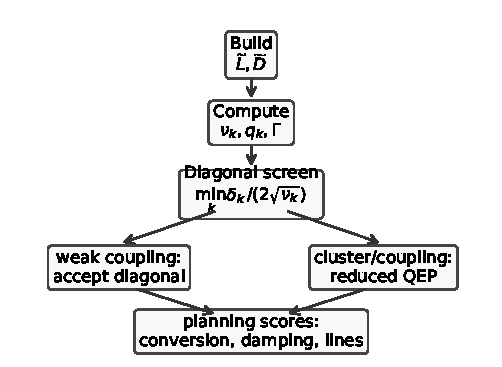
\includegraphics[width=\columnwidth]{figures/fig3_adaptive_workflow.pdf}
\caption{Workflow of the adaptive estimator. The diagonal region is the first screen; second-order perturbation supplies the cheap correction; the reduced QEP is triggered by clustered low-damping modes or strong off-diagonal modal damping.}
\label{fig:workflow}
\end{figure}

\section{Planning With the Damping Margin}

The estimator becomes useful when it ranks actions. Let $a$ denote a planning action: conversion of a synchronous generator to an IBR, addition of virtual damping, addition of virtual inertia, or local controller retuning. Define
\begin{equation}
J(a)=\zeta_{\min}(L(a),M(a),D(a)),
\end{equation}
and, when costs are available,
\begin{equation}
J_c(a)=\frac{\zeta_{\min}(a)-\zeta_{\min}(0)}{\operatorname{cost}(a)}.
\label{eq:costscore}
\end{equation}
The action with highest $J$ is the safest conversion; the action with highest $J_c$ is the most cost-effective improvement.

\subsection{Interpretation of the Planning Score}

The score is defined using the post-action margin rather than only a derivative at the current operating point. A derivative is local. A conversion from synchronous generation to an inverter can be a finite perturbation to inertia, damping, and control states. For small damping additions, a local formula is useful. For finite SG-to-IBR conversion, the estimator should be recomputed after each candidate action.

The distinction between absolute and incremental scores matters. A candidate action can produce a large incremental improvement but still leave the system below the target margin. Conversely, a candidate can yield modest improvement but preserve the margin during a conversion sequence. For decarbonization planning, the safest action can be written as
\begin{equation}
a^\star=\argmin_{a\in\mathcal{A}}\left[\zeta_\star-\zeta_{\min}(a)\right]_+,
\end{equation}
with cost normalization used after safety is satisfied.

\begin{table}[t]
\centering
\caption{Planning quantities and intended use.}
\label{tab:planning}
\begin{tabular}{p{0.28\columnwidth}p{0.58\columnwidth}}
\toprule
Quantity & Use\\
\midrule
$\zeta_{\min}(a)$ & Safety of finite conversion or reinforcement\\
$\Delta\zeta_{\min}/\operatorname{cost}$ & Cost-effective damping or inertia placement\\
$\partial\zeta_{\min}/\partial w_e$ & Local line-reinforcement screening\\
$\partial\nu_k/\partial w_e$ & Frequency mechanism, not final ranking\\
$q_k(i)^2$ & Modal participation diagnostic\\
\bottomrule
\end{tabular}
\end{table}

\subsection{Controller-Aware Graph Reconfiguration}

Weak-node and weak-link scores are local objects. A graph reconfiguration problem asks how to combine them under a cost budget. The first step is a matrix taxonomy of the available levers. Let $b_{ij}=e_i-e_j$ and define
\begin{align}
\mathcal{L}_{\rm all}
&=\operatorname{span}\{b_{ij}b_{ij}^T:1\le i<j\le n\},\\
\mathcal{D}_{\rm sh}
&=\{\diag(g):g\in\R^n\}.
\end{align}

\begin{proposition}[Line--shunt action decomposition]
\label{prop:lineshuntdecomp}
As real vector spaces,
\begin{equation}
\operatorname{Sym}(n)=\mathcal{L}_{\rm all}\oplus\mathcal{D}_{\rm sh}.
\label{eq:lineshuntdecomp}
\end{equation}
\end{proposition}
\noindent\emph{Proof.}
The line directions span the symmetric zero-row-sum Laplacian subspace, of dimension $n(n-1)/2$. The shunt space has dimension $n$. A diagonal matrix with zero row sums is zero, so the intersection is trivial and the dimensions add to $\dim\operatorname{Sym}(n)$. \hfill$\square$

This algebra is standard; the use here is as a robustness-lever taxonomy. Given a symmetric perturbation $X$, its line part is the unique zero-row-sum matrix with the same off-diagonal entries as $X$, and the residual diagonal is the shunt part. If the existing edge set is $\mathcal{E}$, then
\begin{equation}
\mathcal{L}_{\rm all}
=\mathcal{L}_{\rm ex}\oplus\mathcal{L}_{\rm new},
\end{equation}
where $\mathcal{L}_{\rm ex}$ is spanned by existing line directions and $\mathcal{L}_{\rm new}$ by candidate new-line directions.

The physically useful consequence is that virtual inertia has a restricted structural location. Since $\Lt=M^{-1/2}LM^{-1/2}$, a local inertia perturbation $E_i=e_ie_i^T$ gives
\begin{equation}
\frac{\partial \Lt}{\partial M_i}
=-\frac{1}{2M_i}(E_i\Lt+\Lt E_i).
\label{eq:inertialeverdecomp}
\end{equation}
The sign in \eqref{eq:inertialeverdecomp} says that increasing inertia lowers normalized stiffness; the support statement below is independent of that sign.

\begin{proposition}[Virtual-inertia lever location]
\label{prop:inertialocation}
For any bus $i$, the inertia-induced perturbation satisfies
\begin{equation}
\frac{\partial \Lt}{\partial M_i}\in
\mathcal{L}_{\rm ex}\oplus\mathcal{D}_{\rm sh},
\label{eq:inertiaexistingshunt}
\end{equation}
and has no component in $\mathcal{L}_{\rm new}$.
\end{proposition}
\noindent\emph{Proof.}
The off-diagonal support of $E_i\Lt+\Lt E_i$ is inherited from the existing network support. Proposition~\ref{prop:lineshuntdecomp} then gives a unique decomposition into existing-edge directions plus a diagonal residual; no new-edge direction is needed. \hfill$\square$

Proposition~\ref{prop:inertialocation} does not make inertia and line reinforcement dynamically equivalent: they move modal stiffness with opposite signs in the conservative screen, and the shunt residual may be the part aligned with the critical mode. It gives a structural taxonomy: reinforce existing lines, add new topology, or add shunt-like virtual inertia/synchronous-condenser support.

The same taxonomy gives a modal classifier for whether topology can substitute for inertia. Let $X_i=-\partial\Lt/\partial M_i=X_i^{\rm ex}+\diag(r_i)$ with $X_i^{\rm ex}\in\mathcal{L}_{\rm ex}$. For a normalized critical network-family mode $q_c$, define
\begin{equation}
s_i=1-\frac{|r_i^Tq_c|}{\norm{r_i}+\varepsilon_{\rm reg}}.
\label{eq:modalsubstitutability}
\end{equation}
A high $s_i$ means that the shunt residual is nearly invisible to the critical mode, so existing-line actions are a plausible substitute. A low $s_i$ means that the shunt component is aligned with the critical mode, so inertia or synchronous-condenser support is structurally harder to replace by line-only actions. The small $\varepsilon_{\rm reg}>0$ only handles the zero-residual case. This classifier is a design diagnostic, not yet a validated full-ANDES planner.

The scalar score in \eqref{eq:modalsubstitutability} is only the projection of a larger object. For every retained network-family mode $q_k$, define the node--mode substitutability spectrum
\begin{equation}
s_{i,k}
=1-\frac{|r_i^Tq_k|}
{\norm{r_i}\norm{q_k}+\varepsilon_{\rm reg}},
\qquad
S_{\rm sub}=[s_{i,k}]_{i,k}.
\label{eq:modalsubstitutabilityspectrum}
\end{equation}
The same bus can therefore be line-substitutable for one mode and equipment-requiring for another. This is the structural reason why one-number weak-node scores can lose the mechanism needed for planning: they say where a mode participates, but not whether the repair should be copper, new topology, or local shunt/inertia support. A structural random-graph audit reported in the project ledger found that mode-dependent node rankings disagreed in all $60$ tested random graphs, that the distinction persisted among candidate critical modes, and that in about $98\%$ of the tested graphs the top node for at least one candidate critical mode differed from the top node for the single selected critical mode. These numbers are not full-ANDES evidence; they motivate using $S_{\rm sub}$ as the object to validate, rather than collapsing it prematurely to a scalar.

The same spectrum can be projected onto planning categories. If a Fiedler partition divides the buses into two areas, then the existing-line space splits into intra-area and inter-area directions,
\begin{equation}
\mathcal{L}_{\rm ex}
=\mathcal{L}_{\rm intra}\oplus\mathcal{L}_{\rm inter}.
\label{eq:arealeversplit}
\end{equation}
Writing $X_i^{\rm ex}=X_i^{\rm intra}+X_i^{\rm inter}$ gives the mode-dependent inter-area share
\begin{equation}
\alpha_{i,k}^{\rm inter}
=
\frac{|q_k^TX_i^{\rm inter}q_k|}
{|q_k^TX_i^{\rm ex}q_k|+\varepsilon_{\rm reg}}.
\label{eq:interareashare}
\end{equation}
Large $\alpha_{i,k}^{\rm inter}$ means that the line-substitutable part of the local inertia action mainly lives in corridors between areas; small $s_{i,k}$ with large inter-area share says that the corridor is structurally important but still cannot fully replace local equipment for that mode. In preliminary six-bus structural checks, this projection separated corridor buses from within-area buses. That observation is used only as a diagnostic template until it is repeated on calibrated IEEE39 cases.

There is also a complex-admittance version of the same taxonomy. Over the complex symmetric matrix space,
\begin{equation}
\operatorname{Sym}_{\C}(n)
=\mathcal{L}_{\rm all}^{\C}\oplus\mathcal{D}_{\rm sh}^{\C},
\label{eq:ybusdecomp}
\end{equation}
where complex line directions represent series admittance changes and $\mathcal{D}_{\rm sh}^{\C}$ represents shunt admittance. This is the $Y$-bus sister of Proposition~\ref{prop:lineshuntdecomp}: it supports a copper-versus-reactive-compensation taxonomy for voltage/reactive planning. It should not be confused with the inertia result in Proposition~\ref{prop:inertialocation}; inertia enters the dynamic normalization, while the complex $Y$-bus decomposition organizes line admittance and shunt compensation such as capacitors or STATCOMs.

The planning interpretation is a damping-aware hosting-capacity screen. For a proposed SG-to-IBR conversion at bus $i$, let $\mathcal{A}_i$ be the admissible local repair set containing existing-line reinforcement, candidate new lines, shunt/STATCOM or synchronous-condenser support, and controller retuning. A local damping-hosting capacity can be written as
\begin{equation}
\begin{aligned}
H_i^{\rm damp}
=\sup_{\rho\in[0,1]}\{\rho:\ 
&\exists u\in\mathcal{A}_i,\ 
m_H(\rho,i,u)\ge m_\star,\\
&c^T|u|\le B\}.
\end{aligned}
\label{eq:dampinghostingcapacity}
\end{equation}
Equation~\eqref{eq:dampinghostingcapacity} is not a thermal or voltage hosting metric. It asks how much conversion can be hosted while preserving the composite phase--damping--control-resonance margin. The novelty, if it survives the literature and ANDES gates, would not be generic hosting capacity; it would be the mode-resolved decision of whether a low-inertia conversion is repairable by existing copper, requires new topology, or requires local equipment/control support.

Let $u$ collect admissible changes in existing lines, candidate new lines, shunt/inertia support, damping, and controller settings:
\begin{equation}
u=\left[u_{\rm ex},u_{\rm new},u_{\rm sh},u_M,u_D,u_\kappa\right]^T .
\label{eq:levervector}
\end{equation}
The corresponding first-order matrix action has the structured form
\begin{equation}
\begin{aligned}
\Delta \Lt(u)=&
\sum_{e\in\mathcal{E}}u_{{\rm ex},e}G_e
+\sum_{e\notin\mathcal{E}}u_{{\rm new},e}G_e\\
&+\sum_i u_{{\rm sh},i}E_i
+\Delta \Lt_M(u_M),
\end{aligned}
\label{eq:levermatrix}
\end{equation}
where $G_e=b_eb_e^T$ in normalized coordinates and $\Delta\Lt_M$ is the virtual-inertia perturbation in \eqref{eq:inertialeverdecomp}. Equation~\eqref{eq:levermatrix} is the matrix-geometric representation of the planning levers: topology, new topology, shunt/inertia, damping, and control enter the same NEP but occupy different structured directions.

For a fixed tracked pole $s_k$, NEP sensitivity gives a first-order pole-motion map
\begin{equation}
\Delta s_k\approx J_k u,\qquad
J_k=\left[\frac{\partial s_k}{\partial p_1},\ldots,
\frac{\partial s_k}{\partial p_r}\right].
\label{eq:polemotionmap}
\end{equation}
In real pole coordinates, $J_k$ maps feasible graph and control actions into a cone of possible pole motions in the complex plane. The damping-ratio gradient then gives
\begin{equation}
\Delta\zeta_k\approx g_k^T u,\qquad
g_k=\left[\frac{\partial\zeta_k}{\partial p_1},\ldots,
\frac{\partial\zeta_k}{\partial p_r}\right]^T .
\end{equation}
Thus a local cost-constrained reconfiguration can be posed either as a max-margin problem,
\begin{align}
\max_{u,t}\quad & t\\
\text{s.t.}\quad &
\zeta_k+g_k^Tu\ge t,\quad k\in\mathcal{K},\nonumber\\
& c^T|u|\le B,\qquad u\in\mathcal{U},
\label{eq:reconfiglp}
\end{align}
where $\mathcal{K}$ is the set of protected oscillatory modes, $c$ is an action-cost vector, and $\mathcal{U}$ encodes engineering limits. A hidden-resonance constraint can be added by linearizing the control-pole distance:
\begin{equation}
d_{kj}^{\rm ctrl}+h_{kj}^Tu\ge d_{\min},
\qquad
h_{kj}=\nabla_u d_{kj}^{\rm ctrl}.
\label{eq:hiddenconstraint}
\end{equation}
or as a minimum-cost hidden-margin repair problem,
\begin{align}
\min_{u}\quad &
c_{\rm ex}^T|u_{\rm ex}|+
c_{\rm new}^T|u_{\rm new}|+
c_{\rm sh}^T|u_{\rm sh}|
\nonumber\\
&+
c_M^T|u_M|+
c_D^T|u_D|+
c_\kappa^T|u_\kappa|
\nonumber\\
\text{s.t.}\quad &
\zeta_k+g_k^Tu\ge \zeta_\star,\quad k\in\mathcal{K},
\nonumber\\
&
d_{kj}^{\rm ctrl}+h_{kj}^Tu\ge d_\star,\quad
(k,j)\in\mathcal{R},
\nonumber\\
& u\in\mathcal{U}.
\label{eq:hiddenrepair}
\end{align}
Here $\mathcal{R}$ contains the network/control pole pairs that are close enough to matter. Equations \eqref{eq:polemotionmap}--\eqref{eq:hiddenrepair} are not yet a validated planner. They define the matrix-geometric version of the proposed framework: topology and controller actions generate a pole-motion cone, damping-margin safety is a half-space in that cone, and hidden control-resonance safety is a distance constraint to condensed-control poles. This is the intended route from weak-element diagnosis to graph configuration optimization.

The feasible action set in \eqref{eq:reconfiglp}--\eqref{eq:hiddenrepair} is often a polytope in the coordinates of \eqref{eq:levervector}, but the true margin objective is not a linear program. The global map
\begin{equation}
u\mapsto m_H(u)
=\min\{m_\phi(u),m_\zeta(u),m_c(u)\}
\label{eq:nonconvexmarginmap}
\end{equation}
is generally nonsmooth because the active mode, active line-angle constraint, or nearest control pole can change. Thus the safe use of the polytope is local: after fixing the active modes and pole pairs, first-order sensitivity gives the linearized problem
\begin{equation}
\max_{u\in\mathcal{P}} g_H^Tu,
\qquad
\mathcal{P}=\{u\in\mathcal{U}:c^T|u|\le B\},
\label{eq:localpolytope}
\end{equation}
where $g_H=\nabla_u m_H$ for the currently active margin. The optimum of \eqref{eq:localpolytope} occurs at an extreme point of $\mathcal{P}$ when the linearized model is valid, so the first-order repair often selects a pure lever or a sparse mixture. This is only a local screening statement. It should not be read as a global convexity theorem for damping-margin planning.

\subsection{SG-to-IBR Conversion}

A single conversion can be modeled at the reduced level by changing the inertia and damping assigned to the candidate bus:
\begin{equation}
M_i\leftarrow M_{\rm IBR},\qquad D_i\leftarrow D_{\rm IBR}.
\end{equation}
The exact mapping depends on whether the replacement is grid-following or grid-forming. A grid-following inverter should not be treated as a perfect nodal damping element in final models; the approximation is a planning surrogate that must be validated against full IBR state-space models. The value of the estimator is that it screens many candidates cheaply before full eigensolve or time-domain analysis.

The baseline comparisons are essential. A Fiedler-participation rule ranks buses by $q_2(i)^2$. A frequency-participation rule ranks buses by participation in the highest-frequency mode. An inertia heuristic ranks buses by current $M_i$. None of these directly optimizes \eqref{eq:zeta}. The proposed rule ranks by post-conversion margin. If a simple proxy matches the exact margin in a benchmark, that result should be reported; if it fails, the failure is the justification for the spectral estimator.

\subsection{Damping and Virtual-Inertia Placement}

For small additions $\Delta D_i$ or $\Delta M_i$, a first-order placement score can be derived from the diagonal region. If $D_i$ changes while $M$ and $L$ are fixed,
\begin{equation}
\frac{\partial \delta_k}{\partial D_i}=\frac{q_{k,i}^2}{M_i},
\end{equation}
and hence
\begin{equation}
\frac{\partial \zeta_k}{\partial D_i}\approx
\frac{q_{k,i}^2}{2M_i\sqrt{\nu_k}}.
\label{eq:dampingplace}
\end{equation}
This expression gives a transparent damping-placement score, but it must be applied to the mode that determines $\zeta_{\min}$ and corrected when modal coupling is strong. Virtual inertia is more delicate because it changes the normalization, modal frequencies, and damping geometry simultaneously. Therefore, inertia placement should be evaluated by recomputing the adaptive estimator after the candidate action rather than by relying solely on a closed-form scalar score.

For infinitesimal inertia actions, however, Appendix B gives the closed-form score
\begin{equation}
\frac{\partial\zeta_k}{\partial M_i}
=\frac{1}{2\sqrt{\nu_k}}\frac{\partial\delta_k}{\partial M_i}
+\frac{\delta_k q_{k,i}^2}{4M_i\sqrt{\nu_k}},
\label{eq:inertiascore}
\end{equation}
with $\partial\delta_k/\partial M_i$ in \eqref{eq:deltadmi}. Unlike \eqref{eq:dampingplace}, this derivative is sign-indefinite: inertia changes both the graph frequency and the modal damping geometry.

A useful sign test follows when the local damping-per-inertia ratio
$\bar d_i=D_i/M_i$ is held fixed during an infinitesimal inertia change. This
removes the trivial effect in which fixed physical damping is diluted by larger
inertia. Let
\begin{equation}
G_i=\frac{\partial \Lt}{\partial M_i}
=-\frac{E_i\Lt+\Lt E_i}{2M_i},
\end{equation}
where $E_i=e_ie_i^T$. For a simple mode $k$,
\begin{equation}
\frac{\partial \nu_k}{\partial M_i}=-\frac{\nu_k q_{k,i}^2}{M_i},
\end{equation}
and the modal-damping rotation term is
\begin{equation}
\left(\frac{\partial\delta_k}{\partial M_i}\right)_{\rm rot}
=2\sum_{\ell\neq k}
\frac{(q_\ell^TG_iq_k)(q_\ell^T\Dt q_k)}{\nu_k-\nu_\ell}.
\label{eq:inertiadeltarot}
\end{equation}
Thus the diagonal modal damping-ratio derivative is
\begin{equation}
\frac{\partial\zeta_k}{\partial M_i}
=\frac{1}{2\sqrt{\nu_k}}
\left(\frac{\partial\delta_k}{\partial M_i}\right)_{\rm rot}
+\frac{\delta_k q_{k,i}^2}{4M_i\sqrt{\nu_k}}.
\label{eq:inertiasign}
\end{equation}
The second term in \eqref{eq:inertiasign} is positive, but the rotation term can be negative. Therefore, increasing inertia can reduce the diagonal damping-ratio screen whenever
\begin{equation}
\left(\frac{\partial\delta_k}{\partial M_i}\right)_{\rm rot}
<-\frac{\delta_k q_{k,i}^2}{2M_i}.
\label{eq:inertiareversal}
\end{equation}
This is not a claim that inertia is harmful in general. It is a sign condition showing that, under non-proportional damping, inertia placement is not monotone in the damping margin.

\begin{table}[t]
\centering
\caption{Inertia-reversal Monte Carlo check. A reversal means that increasing $M_i$ lowers the damping margin under a finite-difference perturbation.}
\label{tab:inertiareversal}
\begin{tabular}{lccc}
\toprule
Assumption & Tests & Full rev. & Diag+full rev.\\
\midrule
Fixed $D_i/M_i$ & 16229 & 7694 & 5447\\
Fixed $D_i$ & 16229 & 11054 & 8425\\
\bottomrule
\end{tabular}
\end{table}

Table~\ref{tab:inertiareversal} reports a reproducible random-graph audit. The fixed-$D_i$ case is included as a control because it contains direct damping dilution. The fixed-$D_i/M_i$ case is the nontrivial check: in the strongest five-node example, \eqref{eq:inertiasign} predicts $\partial\zeta_k/\partial M_i=-0.0373$, the matched-mode finite difference gives $-0.0397$, and the full-QEP damping-margin finite difference is also negative ($-0.106$). The larger full-QEP derivative is not a contradiction. Equation \eqref{eq:inertiasign} is a diagonal matched-mode sensitivity, while the full-QEP margin also includes off-diagonal modal coupling and possible movement of the identity of the critical mode. In this example, the coupled system amplifies the same sign reversal detected by the diagonal formula. This supports the mechanism but remains a reduced-model result; it has not yet been validated on calibrated ANDES IBR dynamics.

\subsection{Progressive Conversion}

A practical transition is not a single conversion; it is a sequence. Let $\mathcal{C}$ be the set of synchronous generators still eligible for conversion. At step $m$, define
\begin{equation}
i_m=\argmax_{i\in\mathcal{C}}\zeta_{\min}(M^{(m,i)},D^{(m,i)},L^{(m)}),
\end{equation}
where $(M^{(m,i)},D^{(m,i)},L^{(m)})$ is the model after converting candidate $i$ on top of the previous $m-1$ conversions. This greedy rule should be compared against a fixed merit order, random order, inertia order, and modal-participation order.

Progressive conversion is important because single-action ranking can overstate robustness. A bus that is safe to convert first may become unsafe after another conversion changes the critical mode. The benchmark should report the full margin trajectory versus IBR penetration, not only the first selected bus. If the greedy rule fails at a certain penetration level, that failure is a useful result: it identifies where local planning must be replaced by combinatorial or robust optimization.

\section{Damping-Aware Line Reinforcement}

The old line map is the Rayleigh sensitivity of the inertial-Laplacian eigenvalue:
\begin{equation}
\frac{\partial \nu_k}{\partial w_{ij}}=
\left(\frac{q_{k,i}}{\sqrt{M_i}}-\frac{q_{k,j}}{\sqrt{M_j}}\right)^2.
\label{eq:rayleigh}
\end{equation}
This formula is useful, but it answers the wrong planning question if used alone. It says which line raises modal stiffness or frequency. It does not say which line raises damping margin.
Equivalently, the unnormalized Laplacian perturbation is
$\partial L/\partial w_{ij}=(e_i-e_j)(e_i-e_j)^T$, while the perturbation used in modal formulas is the inertia-normalized matrix
\begin{equation}
\frac{\partial \Lt}{\partial w_{ij}}=
M^{-1/2}(e_i-e_j)(e_i-e_j)^TM^{-1/2}.
\label{eq:normlinepert}
\end{equation}

The reason is immediate from the diagonal formula:
\begin{equation}
\zeta_k=\frac{\delta_k}{2\sqrt{\nu_k}}.
\end{equation}
Differentiating with respect to a line weight $w_e$ gives
\begin{equation}
\frac{\partial \zeta_k}{\partial w_e}=
\frac{1}{2\sqrt{\nu_k}}\frac{\partial \delta_k}{\partial w_e}
-\frac{\delta_k}{4\nu_k^{3/2}}\frac{\partial \nu_k}{\partial w_e}.
\label{eq:zetaline}
\end{equation}
The second term is negative when reinforcement increases $\nu_k$. Thus, a line can raise frequency while reducing damping ratio if the first term does not compensate. Fig.~\ref{fig:tradeoff} illustrates the same mechanism in pole coordinates: increasing $|\omega|$ while holding $-\sigma$ fixed lowers $\zeta=-\sigma/\sqrt{\sigma^2+\omega^2}$.

\begin{figure}[t]
\centering
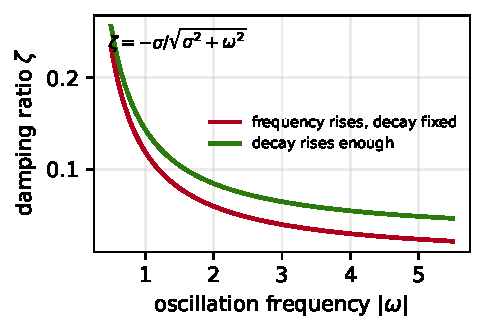
\includegraphics[width=\columnwidth]{figures/fig4_line_tradeoff.pdf}
\caption{Frequency--damping tradeoff. If a line reinforcement increases oscillation frequency without increasing decay rate enough, damping ratio decreases. This is not a topological Braess paradox; it is the definition of damping ratio.}
\label{fig:tradeoff}
\end{figure}

For a simple eigenvalue of $\Lt$, the derivative of modal damping is
\begin{equation}
\frac{\partial \delta_k}{\partial w_e}=
q_k^T\frac{\partial \Dt}{\partial w_e}q_k
+2\sum_{\ell\neq k}
\frac{(q_\ell^T\frac{\partial \Lt}{\partial w_e}q_k)(q_\ell^T\Dt q_k)}
{\nu_k-\nu_\ell}.
\label{eq:deltaline}
\end{equation}
If line reinforcement affects only $L$, the first term is zero, but the second term can be nonzero because the eigenvectors rotate relative to the damping matrix. This is the precise mechanism by which non-proportional damping changes line-ranking decisions.

For the exact QEP, let $s$ be a simple critical root with right and left eigenvectors $v$ and $y$:
\begin{equation}
P(s)v=0,\qquad y^\ast P(s)=0.
\end{equation}
The normalization of $v$ and $y$ is arbitrary because it cancels between numerator and denominator in the sensitivity expression; the only requirement is $y^\ast P'(s)v\neq0$ for a simple root.
For a scalar parameter $\rho$,
\begin{equation}
\frac{ds}{d\rho}=
-\frac{y^\ast\left(s\frac{\partial \Dt}{\partial\rho}+\frac{\partial \Lt}{\partial\rho}\right)v}
{y^\ast(2sI+\Dt)v},
\label{eq:qepsens}
\end{equation}
assuming the coefficient of $s^2$ is fixed in the chosen coordinates. If $s=\sigma+j\omega$ and $ds/d\rho=a+jb$, then
\begin{equation}
\frac{d\zeta}{d\rho}=
\frac{\sigma\omega b-\omega^2a}{|s|^3}.
\label{eq:zetasens}
\end{equation}
Equations \eqref{eq:qepsens}--\eqref{eq:zetasens} define the damping-aware line map. The frequency map \eqref{eq:rayleigh} remains useful for mechanism interpretation, but the ranking variable is $\partial\zeta_{\min}/\partial w_e$ or a finite post-action $\Delta\zeta_{\min}$.

\subsection{Finite-Difference Validation}

Before using \eqref{eq:qepsens} operationally, the analytic sensitivity should be checked against finite differences. For edge $e=(i,j)$ with base weight $w_e$, define
\begin{equation}
\Delta_e^{\rm FD}(\epsilon)=
\frac{\zeta_{\min}(w_e(1+\epsilon))-\zeta_{\min}(w_e)}{\epsilon w_e}.
\end{equation}
The perturbation should preserve Laplacian row sums:
\begin{equation}
\Delta L_e=\epsilon w_e(e_i-e_j)(e_i-e_j)^T.
\end{equation}
The analytic sensitivity should converge to $\Delta_e^{\rm FD}$ as $\epsilon$ decreases until roundoff dominates. If the identity of the critical eigenvalue changes during the perturbation, the line should be flagged as a nonsmooth ranking point rather than forced into a smooth derivative.

\subsection{Why Frequency-Only Ranking Can Fail}

The frequency map \eqref{eq:rayleigh} is nonnegative in the scalar lossless model:
\begin{equation}
\frac{\partial\nu_k}{\partial w_e}\geq 0.
\end{equation}
Thus reinforcement increases or preserves modal stiffness. The mistake is to equate stiffness with damping margin. For a lightly damped pole, $\omega\approx\sqrt{\nu_k}$ while $\sigma$ is set by damping and modal rotation. If $\omega$ increases while $\sigma$ is fixed, $\zeta$ decreases. If eigenvector rotation moves the mode toward lower-damped buses, $\sigma$ can also become less negative. The corrected map therefore decomposes reinforcement into a frequency term and a modal-damping-rotation term.

\section{Benchmark Validation Protocol}

The decisive validation target is the IEEE 39-bus New England system in ANDES \cite{andesdocs}. A final submission should not rely only on random graphs or low-order examples. The intended validation pipeline is as follows.

\subsection{System Setup}

The base case should be initialized with a solved power flow. Synchronous machines should use documented dynamic models available in ANDES, such as GENROU or the closest supported equivalent. IBR penetration should be introduced by replacing a fraction $\rho$ of synchronous capacity with documented inverter models. Grid-following replacements should include PLL dynamics where available. Grid-forming replacements should use droop or virtual-synchronous-machine models where available. Controller gains should be documented and should not be hand-tuned to make the proposed method look better.

\subsection{Experiments}

Experiment A compares margin estimators. For each penetration level $\rho$, compute the full small-signal poles using ANDES, then compare the homogeneous formula, Fiedler-only formula, diagonal all-mode estimate, and adaptive reduced QEP.

Experiment B tests the coupling diagnostic. The expected outcome is not that the diagonal estimate always fails or always succeeds. The expected outcome is that the diagnostic predicts when it can be trusted.

Experiment C ranks SG-to-IBR conversions. Each candidate conversion is evaluated by the adaptive estimator and by full eigensolve. Baselines include Fiedler participation, highest-frequency participation, and inertia-only heuristics.

Experiment D tests multi-node conversion. Greedy conversion by post-action damping margin is compared against random conversion and heuristic merit orders. Failures must be reported, especially if interactions make the greedy rule unreliable.

Experiment E evaluates line reinforcement. Rank lines by $\partial\nu/\partial w$, finite-difference $\Delta\zeta_{\min}$, and analytic QEP sensitivity. The key test is whether frequency-only reinforcement disagrees with damping-aware reinforcement and whether the analytic sensitivity predicts the full eigensolve.

\subsection{Extracting Reduced Quantities From ANDES}

The ANDES bridge must be documented carefully. The full ANDES state matrix contains device states, algebraic variables, controllers, and possibly load or network dynamics. The reduced spectral model requires $L$, $M$, and $D$ or their best physically justified equivalents.

The extraction should proceed in two levels. Level 1 constructs the second-order surrogate. The active-power Jacobian with respect to bus angles gives the stiffness matrix corresponding to $L$ under the assumptions of \eqref{eq:swing}. Synchronous-machine inertia and virtual inertia terms define $M_i$. Mechanical damping, droop, and equivalent local damping define $D_i$ only when the mapping is physically meaningful. Level 2 compares that surrogate against the full ANDES linearization with IBR controller states. Failure at Level 2 would not invalidate the mathematics of the estimator; it would delimit the regime where a scalar $L,M,D$ surrogate is insufficient.

\begin{table}[t]
\centering
\caption{Pre-registered ANDES validation matrix.}
\label{tab:andes}
\begin{tabular}{p{0.31\columnwidth}p{0.55\columnwidth}}
\toprule
Experiment & Metric\\
\midrule
Estimator accuracy & Median and 95th-percentile error vs full eigensolve\\
Coupling trigger & Precision/recall of diagonal-failure detection\\
Conversion ranking & Top-1 and top-3 agreement with full eigensolve\\
Multi-conversion & Margin trajectory vs penetration level\\
Line sensitivity & Correlation and top-$k$ overlap with finite differences\\
Surrogate fidelity & Scalar model poles vs full ANDES IBR poles\\
\bottomrule
\end{tabular}
\end{table}

\subsection{Success Criteria}

The method should be judged by pre-registered criteria:
\begin{itemize}
\item median and 95th-percentile error of margin estimates,
\item fraction of cases where the adaptive estimator identifies the correct critical mode or cluster,
\item top-$k$ accuracy of conversion ranking,
\item agreement between analytic and finite-difference line sensitivities,
\item failure cases and their mechanisms.
\end{itemize}
If the adaptive estimator fails at high IBR penetration, that result should be included. The value of the paper is a calibrated method, not a universal claim.

\subsection{Decision Gates for Claim Strength}

The final benchmark should assign each contribution a claim level before submission. The highest level is an empirical contribution: the method is validated against full ANDES poles over the stated operating range and beats the registered baselines. The middle level is a theoretical or diagnostic contribution: the mathematics is correct and the mechanism is visible, but benchmark advantage is narrow or case-dependent. The lowest level is a cautionary result: the proposed idea identifies a failure mode of simpler reasoning, but it is not strong enough to headline the paper.

For C1, the empirical level requires that the modal points in the $(\nu,\delta)$ plane predict safe and unsafe cases in the commuting or weakly coupled regime, and that the same plot visually explains at least one non-proportional failure. If the plot is only exact in toy proportional cases, C1 should be framed as theory background plus visualization, not as a benchmark contribution.

For C2, the empirical level requires that the adaptive estimator reduce error or computational burden relative to full eigensolve and relative to the diagonal screen in the cases where the coupling diagnostic fires. If the diagonal all-mode formula is already accurate on every IEEE 39 case, the reduced QEP should be demoted to a safeguard for degenerate or artificially clustered modes. This would still be a valid result, but it would change the title and contribution ordering.

For C3, the empirical level requires low regret, not only high correlation. A conversion ranking that is usually correlated with the full eigensolve but occasionally chooses an action with a much lower margin is not operationally acceptable. The correct fallback claim would be that the estimator provides a screening list for full eigensolve, not a standalone planner.

For C4, the empirical level requires two checks. First, analytic sensitivity must match finite differences when the critical pole is smooth. Second, damping-aware ranking must differ materially from frequency-only ranking in at least some realistic operating points. If both rankings agree on IEEE 39, the result should be stated as a theoretical correction that prevents a known category error rather than as evidence of a frequent planning reversal.

\begin{table}[t]
\centering
\caption{Claim levels used after benchmark validation.}
\label{tab:claimlevels}
\begin{tabular}{p{0.23\columnwidth}p{0.64\columnwidth}}
\toprule
Level & Meaning\\
\midrule
Empirical contribution & Verified against full benchmark poles and stronger than registered baselines\\
Diagnostic contribution & Mathematically correct and mechanism-clear, but benchmark advantage is case-dependent\\
Cautionary result & Useful for avoiding a wrong inference, but not a standalone planning method\\
Rejected claim & Control comparison or mechanism check fails\\
\bottomrule
\end{tabular}
\end{table}

\subsection{Negative Controls}

The benchmark should include controls that are expected to fail. These controls are not straw men; they are the reason the proposed method is needed. A Fiedler-only estimate should fail whenever the damping-critical mode is not the lowest nonzero graph frequency. A homogeneous damping formula should fail when IBR conversion creates large variation in $D_i/M_i$. A frequency-only line map should fail whenever reinforcement raises $\nu_k$ while modal damping does not rise enough to preserve $\zeta_k$. A low-frequency QEP should fail when the least damped mode is outside the retained frequency band.

Reporting these controls prevents a common source of false positives. If the proposed estimator beats only an obviously wrong control but not the diagonal all-mode screen, then the central claim is not the reduced QEP. If the damping-aware line map beats frequency sensitivity but not finite-difference full eigensolve, then the analytic implementation is wrong or the pole is nonsmooth. Each negative control therefore has a paired diagnostic that identifies whether the failure is caused by the baseline assumption, the proposed approximation, or the reduced surrogate itself.

\begin{table*}[t]
\centering
\caption{Contribution status and required validation.}
\label{tab:status}
\begin{tabular}{p{0.17\textwidth}p{0.24\textwidth}p{0.22\textwidth}p{0.19\textwidth}}
\toprule
Component & What is established & What is not established & Required next check\\
\midrule
Damping region & Exact for commuting damping; first-order screen for weak non-proportional damping & Novelty of the region language for IBR planning & Literature search and IEEE 39 modal plots\\
Adaptive estimator & Synthetic tests separate diagonal-safe and QEP-needed regimes & Universal diagnostic threshold & ANDES full eigensolve comparison\\
Conversion ranking & Planning score is well-defined by post-action $\zeta_{\min}$ & Multi-node interaction robustness & Greedy conversion sweep on IEEE 39\\
Damping-aware line map & Mechanism and QEP sensitivity formulas are derived & Analytic implementation vs finite differences & Line perturbation sensitivity in ANDES\\
\bottomrule
\end{tabular}
\end{table*}

\section{Claim Calibration and Evidence Map}

The proposed paper has to survive a strict novelty and mechanism audit. This section states how each contribution should be defended and what evidence would be required in a final submission.

\subsection{C1 Is a Region Framework, Not a New Scalar Formula}

The formula $\zeta_k=\delta_k/(2\sqrt{\nu_k})$ in the commuting case is a standard modal result. The contribution is not the formula. The contribution is the use of the $(\nu,\delta)$ plane as a planning coordinate for heterogeneous IBR damping, together with the statement that this coordinate is exact only in the commuting case and diagnostic otherwise. The consensus-region analogy is useful because it changes the question from ``which graph eigenvalue is critical?'' to ``which modal points lie outside the admissible damping region?'' This avoids the common mistake of treating $\lambda_2$ as a damping margin.

Fig.~\ref{fig:region} therefore includes two visual checks. The commuting case shows where the region is an exact margin certificate. The non-proportional panel shows the failure mode: a diagonal modal point can lie above the target curve while the coupled QEP pole falls below the margin. This makes C1 a boundary-aware framework rather than a standalone novelty claim.

\subsection{C2 Is a Mode-Selection Rule, Not Generic Model Reduction}

Reduced QEPs are well known. The estimator's claim is the selection logic. Low-frequency truncation is natural in inter-area oscillation analysis, but the damping margin is the minimum damping ratio over all oscillatory modes. A high-frequency mode can be less damped than a Fiedler mode if $\delta_k$ is small enough. Conversely, a low-frequency mode can be safe if its modal damping is large. The reduced model should therefore be built from low estimated damping and strong modal coupling, not from frequency alone.

The evidence needed for this claim is an ablation table. Let $\zeta_{\rm full}$ be the reference. Compare:
\begin{align}
e_{\rm hom} &= |\zeta_{\rm hom}-\zeta_{\rm full}|/\zeta_{\rm full},\\
e_{\rm Fiedler} &= |\zeta_{2}-\zeta_{\rm full}|/\zeta_{\rm full},\\
e_{\rm freqQEP} &= |\zeta_{\rm lowfreqQEP}-\zeta_{\rm full}|/\zeta_{\rm full},\\
e_{\rm adapt} &= |\zeta_{\rm adapt}-\zeta_{\rm full}|/\zeta_{\rm full}.
\end{align}
The adaptive estimator is justified only if $e_{\rm adapt}$ improves the cases where simple baselines fail and if the diagnostic explains the improvement.

\subsection{C3 Is a Planning Rule With a Full-Eigensolve Reference}

The conversion and placement contribution should be judged by ranking accuracy, not only by correlation. A high correlation can hide top-action mistakes. Let $r_{\rm est}(i)$ and $r_{\rm full}(i)$ be the estimated and true ranks of candidate action $i$. Useful metrics include top-1 hit rate, top-3 overlap, Kendall rank correlation, and regret:
\begin{equation}
\operatorname{regret}=
\zeta_{\min}(a^\star_{\rm full})-\zeta_{\min}(a^\star_{\rm est}).
\end{equation}
Regret is especially important for planning. If several actions are nearly tied, a wrong top-1 selection may have negligible regret. If the wrong action collapses the margin, the ranking method is not acceptable even with high average correlation.

\subsection{C4 Is a Damping Sensitivity, Not a Braess Claim}

The line-reinforcement contribution is easiest to overstate. The paper should not say that reinforcement creates a new dynamic Braess paradox unless a topological feedback mechanism is demonstrated. The defensible claim is simpler and stronger: frequency-only line ranking can be wrong because damping ratio depends on both decay and frequency. The exact QEP sensitivity gives the derivative of the pole, and \eqref{eq:zetasens} converts it to a damping-ratio derivative.

The NEP reinforcement audit refines this boundary. Most observed reinforcement reversals remain geometric or non-resonant damping-ratio effects, but a minority satisfy a stricter network-control resonance test: reinforcement moves a network-family mode toward a PLL-dominated condensed-control pole and the self-energy term dominates the damping decrease. This is a confirmed mechanism in the Mix60/no-PSS audits, not a universal topology law and not the dominant source of global margin loss.

The final line-reinforcement experiment should report three lists for each operating point: top lines by $\partial\nu/\partial w$, top lines by analytic $\partial\zeta/\partial w$, and top lines by finite-difference $\Delta\zeta$. A disagreement between the first and the latter two is the evidence for C4. Agreement between analytic sensitivity and finite difference is the evidence that the formula is implemented correctly.

\begin{algorithm}[t]
\caption{Damping-aware line ranking}
\label{alg:line}
\begin{algorithmic}[1]
\STATE Input: $L,M,D$, edge set $\mathcal{E}$, perturbation size $\epsilon$
\STATE Compute $\zeta_{\min}$ and the critical pole $s$
\FOR{each edge $e=(i,j)\in\mathcal{E}$}
\STATE Build $\partial L/\partial w_e=(e_i-e_j)(e_i-e_j)^T$
\STATE Evaluate analytic $ds/dw_e$ from \eqref{eq:qepsens}
\STATE Convert $ds/dw_e$ to $d\zeta/dw_e$ using \eqref{eq:zetasens}
\STATE Optionally compute finite-difference $\Delta_e^{\rm FD}(\epsilon)$
\ENDFOR
\STATE Rank edges by $d\zeta_{\min}/dw_e$ or finite $\Delta\zeta_{\min}$
\STATE Report $\partial\nu/\partial w_e$ only as a mechanism diagnostic
\end{algorithmic}
\end{algorithm}

\begin{algorithm}[t]
\caption{Greedy SG-to-IBR conversion screening}
\label{alg:conversion}
\begin{algorithmic}[1]
\STATE Input: base model $(L,M,D)$, candidates $\mathcal{C}$, target penetration
\STATE Initialize converted set $\mathcal{S}=\emptyset$
\WHILE{penetration target not reached}
\FOR{each $i\in\mathcal{C}\setminus\mathcal{S}$}
\STATE Apply candidate conversion $i$ to obtain $(L_i,M_i,D_i)$
\STATE Estimate $\widehat{\zeta}_i$ with Algorithm~\ref{alg:adaptive}
\ENDFOR
\STATE Convert $i^\star=\argmax_i\widehat{\zeta}_i$
\STATE Append $i^\star$ to $\mathcal{S}$ and recompute the operating point if required
\ENDWHILE
\STATE Validate the selected sequence against the full eigensolve
\end{algorithmic}
\end{algorithm}

\begin{table}[t]
\centering
\caption{Evidence required before final submission.}
\label{tab:evidence}
\begin{tabular}{p{0.22\columnwidth}p{0.66\columnwidth}}
\toprule
Claim & Required evidence\\
\midrule
C1 region & Modal plots showing safe/unsafe boundary and failures under coupling\\
C2 estimator & Ablation against homogeneous, Fiedler, frequency-QEP, and full eigensolve\\
C3 planning & Top-$k$ ranking, regret, and multi-conversion trajectory\\
C4 line map & Analytic-vs-finite-difference sensitivity and disagreement with frequency-only ranking\\
\bottomrule
\end{tabular}
\end{table}

\section{Discussion}

The proposed framework has three important limits. First, the scalar swing-equation Laplacian is not a full dq-domain inverter-network model. It captures the electromechanical and stiffness geometry used by many spectral power-network studies, but high-order inverter states, current loops, limiters, and dynamic line models can change the relevant modes. The ANDES validation stage is therefore not optional.

Second, the second-order correction is not a universal replacement for a reduced or full eigensolve. It improves the diagonal screen in weak-to-moderate non-proportional regimes and gives an interpretable coupling decomposition, but it can worsen tail errors in strongly coupled or near-degenerate cases. Those cases are exactly why the reduced QEP remains in the workflow.

Third, the line-reinforcement result separates two mechanisms that should not be conflated. If reinforcement raises frequency and lowers damping ratio because decay does not increase enough, the mechanism is ordinary damping-ratio geometry. The Schur-NEP audit confirms a second, narrower mechanism: a network-family mode can be pulled toward a PLL-dominated condensed-control pole, so the self-energy term drives the damping decrease. This resonant mechanism is control-conditional, appears in $40/348$ global-margin-reversal audit records in the Mix60/no-PSS audit, and is absent under the soft-GFL negative control. The paper should therefore say that a control-resonant reinforcement reversal exists and is actionable, not that it dominates line-reinforcement planning or collapses the global margin in this benchmark.

The H-infinity disturbance view and switched-topology Lyapunov view are valuable extensions, but they should not be central in this manuscript. The H-infinity view asks which disturbance shapes excite the reduced system. It is complementary to damping margin but risks reviving poorly defined ``weak pathway'' claims if not controlled carefully. The switched-topology view requires common or multiple Lyapunov functions and dwell-time assumptions; it is a larger thesis direction rather than a clean first paper.

\subsection{Originality Boundaries}

The paper's novelty boundary should be stated plainly. Modal swing-equation formulas under proportional damping, Rayleigh eigenvalue sensitivity, QEP sensitivity, Schur complements, contour NEP solvers, broad stability-region ideas, and eigenvalue perturbation are known. The candidate contribution is not new mathematics in isolation. It is a power-systems contribution: identify the controller-aware rational self-energy as the damping-margin bridge when static nodal damping fails, use it to separate network-family from control-family criticality, and then use second-order perturbation as an interpretable estimator component whose full-ANDES advantage must still be tested against registered baselines.

This boundary matters for peer review. A reviewer can object if the paper appears to claim that $\zeta_k=\delta_k/(2\sqrt{\nu_k})$ or generic QEP sensitivity is new. The defensible claim is that the paper uses the diagonal relation as the zero-order network margin, derives the second-order control-coupling correction for the critical margin pole, and shows when this cheap correction should yield to a reduced QEP. Originality should be judged by the formulation, the control comparisons, and the benchmark results, not by whether every mathematical identity is new.

In final form, each contribution should therefore be labeled as follows. The unifying framework is the spectral-attribution ledger \eqref{eq:intro_unified_object}: network geometry enters through $\Lt$, inertia through $M$, and controller dynamics through the rational self-energy $\Sigma(s)$. The strongest full-ANDES empirical contribution is the controller-aware rational NEP bridge, which reproduces the critical poles and enables mechanism audits that a static scalar bridge cannot perform. The central reduced-model mathematical contribution is the second-order margin correction and rational graph-filter interpretation, verified first in the surrogate QEP and reduced PLL model. The control-resonant reinforcement reversal is a bridge-enabled mechanism, but its current evidence is modal-local and control-conditional. The inertia sign reversal is a reduced-model sign result. The joint inertia--control cross term is a valid local perturbation term, but the first Phase-E0 ANDES gate found no measurable singleton GENROU--PLL case; it must not be treated as an empirical headline unless a physically justified virtual-inertia/control case passes a new gate. Planning and line-reinforcement rankings are applications; they become headline contributions only if ANDES validation shows lower regret or materially different rankings than registered controls.

\subsection{Falsification Criteria}

Three outcomes would weaken the paper and should be reported if observed. First, if the second-order correction is no more accurate than the diagonal all-mode formula on IEEE 39 across relevant IBR penetrations, it should be presented only as an interpretive decomposition. Second, if the reduced PLL or scalar $L,M,D$ surrogate does not track full ANDES IBR poles, the contribution should be reframed as a reduced-model screening method rather than a full IBR stability estimator. Third, if damping-aware line ranking does not differ materially from frequency-only ranking on the benchmark, C4 should be reduced to a theoretical caution rather than a headline application.

These criteria make the manuscript stronger. They state before the benchmark what evidence would consolidate, weaken, or refocus the claims.

\subsection{Final Claim-Readiness Audit}

The current repository includes a final claim audit generated from the versioned validation outputs. Table~\ref{tab:finalaudit} summarizes the status at the close of this draft. The central mathematical and reduced-model claims are supported, and the controller-aware full-ANDES bridge is now validated on three diagnostic cases. The estimator and planning claims over that bridge are not yet supported. This distinction is the intended submission boundary of the manuscript.

\begin{table*}[t]
\centering
\caption{Final claim-readiness audit for the current draft.}
\label{tab:finalaudit}
\scriptsize
\begin{tabular}{@{}p{0.16\textwidth}p{0.29\textwidth}p{0.24\textwidth}p{0.20\textwidth}@{}}
\toprule
Claim & Verified evidence & Control or comparison & Current status\\
\midrule
Damping region
& Exact in commuting damping; paired figure shows non-proportional screen failure.
& Commuting diagonal modal equations versus coupled QEP behavior.
& Theoretical/diagnostic; not a standalone novelty claim.\\
Second-order correction
& IEEE39-derived surrogate median error improves from $0.468\%$ to $0.032\%$; reduced PLL model improves median error from $2.16\%$ to $0.09\%$.
& Full surrogate QEP, diagonal all-mode screen, and reduced-QEP fallback.
& Verified on reduced models; full ANDES IBR validation pending.\\
Adaptive workflow
& Surrogate tails show why fallback is needed: second-order p95 $9.91\%$, reduced-QEP p95 $5.44\%$, adaptive p95 $7.43\%$.
& Always-diagonal, always-second-order, and reduced-QEP baselines.
& Diagnostic workflow; no universal trigger theorem claimed.\\
Controller-aware rational bridge
& NEP-Beyn contour solver reproduces full ANDES critical poles in no-PSS, base, and Mix60, including a 13.7 Hz PLL-family critical mode with $\pi_c=0.853$.
& Full ANDES eigensolve; argument-principle counts match extracted contour zeros.
& Bridge verified for diagnostic cases; estimator accuracy experiments next.\\
SG-to-IBR conversion
& Five derived ANDES IEEE39 cases load, solve power flow, and run eigenanalysis with active GFL/GFM devices; Phase-1 tested 50 case/profile controller audits.
& Device inventory, power-flow/eigenanalysis success, controller-only profiles, and diagnostic removal of retained SG controls.
& Case-construction and calibration audit; final conversion-ranking validation over the NEP bridge remains pending.\\
Mode-resolved lever substitutability
& Line--shunt decomposition and virtual-inertia support result are algebraic; project ledger reports a $60$-graph structural audit where node rankings depend on the mode and scalar collapse loses information in about $98\%$ of graphs.
& Compared against scalar weak-node ranking and single-critical-mode projection.
& Structural planning diagnostic; algebra is classical, novelty is the node--mode copper-versus-equipment taxonomy and it still needs adversarial novelty search plus full-ANDES validation.\\
Damping-aware hosting capacity
& Formulated as a composite-margin feasibility problem over SG-to-IBR conversion level, repair action, budget, and hidden phase--damping--control margin.
& Distinguishes thermal/voltage hosting capacity from damping-margin hosting and requires comparison against Fiedler, inertia-only, and damping-index baselines.
& Proposed application bridge; not yet an empirical hosting-capacity claim.\\
Weak links and reinforcement
& In the IEEE39-derived surrogate, $35/46$ reinforcements raise critical modal stiffness while reducing damping margin.
& Frequency-only reinforcement versus finite post-action damping margin.
& Surrogate planning diagnostic; not yet a full ANDES topology claim.\\
Control-resonant reinforcement reversal
& Schur-NEP sensitivity audit identifies $40/348$ global-margin-reversal audit records as strict resonant cases in Mix60/no-PSS; the largest global case is Line 44 (23--36) with $\Delta\zeta_{\min}=-2.75{\times}10^{-5}$ and C-term dominance.
& Soft-GFL negative control gives zero resonant cases; for matching line/mode pairs, relative pole distance increases from $0.0368$ to $0.9167$ and the control denominator fraction falls from $0.959$ to $0.0789$.
& Mechanism confirmed, control-conditional, minority of reversals, and modal-local in this benchmark; not a dominant global-margin-collapse claim.\\
Hidden control-resonance margin
& Defined by normalized distance from a tracked NEP zero to condensed-control poles, the self-energy denominator fraction, the resolvent bound \eqref{eq:resolventbound}, and the combined damping/distance action margin \eqref{eq:combinedhiddenmargin}.
& Uses the same NEP sensitivity and soft-GFL negative control logic as the resonant reinforcement audit.
& New diagnostic and repair formulation; not yet validated as a system-level collapse predictor or planning certificate.\\
Instability-flow weak elements
& Derived from NEP pole sensitivity, control-pole resolvent expansion, graph/modal line participation, and the local weak-element certificate in Proposition~\ref{prop:localweakelement}.
& Must be compared against power-flow loading, betweenness, Fiedler participation, SCR/impedance, and damping-participation rankings.
& Mathematically local first-order diagnostic; superiority as a practical weak-node/weak-link predictor remains an empirical claim.\\
Protected-resolvent graph-filter shaping
& The bi-orthogonal sensitivity \eqref{eq:protectedsens} gives a common local exchange rate for topology, damping, inertia, and controller retuning; line and damping specializations are \eqref{eq:protectedDsens} and \eqref{eq:protectedlinesens}.
& Gamma robustness gate: physical protection profiles give only $21$--$29\%$ agreement between $S_\zeta$ and $S_g$ rankings; reduced coordination gate supports $w+D$ and $w+M$ packages but kills strong nonlinear synergy as a headline.
& Valid input--output extension and reduced-model planning candidate; flow-feasible dynamic Braess and retrofit LP still require full ANDES/dispatch validation.\\
Local action polytope
& Feasible topology, shunt, inertia, damping, and controller changes can be represented in line--shunt coordinates; local first-order repair reduces to a linearized problem over a polytope.
& Explicitly controlled against the false stronger claim that $\zeta_{\min}$ or $m_H$ is globally convex or smooth.
& Geometry language only; safe as local screening, not a global optimization theorem.\\
Inertia sign reversal
& With fixed $D_i/M_i$, $5447/16229$ perturbations reduce both the diagonal modal screen and the full-QEP damping margin.
& Fixed-$D_i/M_i$ check versus fixed-$D_i$ direct damping-dilution control.
& Reduced-model sign diagnostic; not yet a full ANDES IBR claim.\\
Joint inertia--damping term
& Local perturbation formula shows the cross term between $E^{(D)}$ and $E^{(L)}$; initial Phase-E0 ANDES tests found $0/13$ measurable singleton GENROU--PLL cross cases in Mix60/no-PSS.
& Reduces to the fixed-inertia second-order correction when $\Delta M=0$; E0 compares additive versus additive-plus-cross predictions.
& Theoretical local mechanism; not yet an empirical headline or finite-conversion estimator.\\
\bottomrule
\end{tabular}
\end{table*}

\section{Conclusion}

This paper proposed a controller-aware rational self-energy bridge for damping-margin analysis in inverter-dominated grids. The exact Schur NEP retains the frequency-dependent effect of condensed controller and auxiliary states, while the lower-order spectral model organizes the retained network dynamics through $(\nu_k,\delta_k)$: inertial-Laplacian stiffness and modal damping. In non-proportional IBR regimes, off-diagonal modal damping moves the critical pole away from this diagonal network prediction. The closed-form second-order correction quantifies that movement and gives a network-vs-control decomposition of the damping margin.

The same framework yields planning tools, but those tools are secondary until estimator validation is completed over the controller-aware bridge. SG-to-IBR conversion and damping or inertia placement can be ranked by post-action damping margin rather than by Fiedler participation or connectivity. Line reinforcement should be ranked by damping-margin sensitivity, not by frequency sensitivity alone. The hidden control-resonance margin extends this logic: weak nodes and weak links are elements whose local actions can move poles toward a damping threshold or toward a condensed-control resonance. The resolvent bound explains why this margin is hidden from static scalar reductions: the sensitivity can grow as the network-family pole approaches $\operatorname{spec}(A_{cc})$. The instability-flow construction makes this statement operational by decomposing weak elements into modal participation, control-pole resonance exposure, and first-order damping loss. The protected-resolvent extension adds a second certificate: instead of tracking only pole damping, it tracks protected input--output amplification and reveals when forcing and response are spatially decoupled in a non-normal IBR model. This gives a principled way to compare topology, damping, inertia, and controller-retuning actions in one local exchange-rate language, but current evidence is reduced-model and must not be overstated as a full-ANDES flow-feasible planner. In matrix-geometric terms, admissible topology and control actions generate a pole-motion cone, and local graph reconfiguration becomes a cost-constrained problem over damping-margin, protected-gain, flow, and control-distance constraints. The mode-resolved substitutability spectrum further refines weak-node language: a bus is not simply weak or strong, because it may be copper-substitutable for one mode and equipment-requiring for another. This gives a possible damping-aware hosting-capacity interpretation for SG-to-IBR conversion, but it remains a proposed application bridge until novelty and full-ANDES validation gates are closed. These applications require explicit comparison against existing damping-ratio placement, QEP-sensitivity, impedance/SCR, hosting-capacity, and topology-planning methods before they can become headline claims.

The paper is therefore complete at a stronger methodological-draft level than before: the derivation, reduced-model evidence, IEEE39-derived surrogate checks, ANDES baseline diagnosis, SG-to-GFL/GFM case construction, Phase-1 calibration audit, and Phase-0D controller-aware rational NEP bridge are all documented. The bridge result is the key full-ANDES advance: Beyn contour integration reproduces the full ANDES critical poles in no-PSS, base, and Mix60 cases, including the Mix60 PLL-family critical mode that scalar and fixed-point bridges miss. It also enables a control-resonant reinforcement audit: a minority of Mix60/no-PSS line-reinforcement reversals are driven by controller self-energy as network modes move toward PLL-dominated condensed-control poles, while the mechanism disappears under the soft-GFL negative control. This is a confirmed modal-local mechanism, not a global-margin-collapse claim. The manuscript is still not complete as a final IEEE Transactions empirical submission. The next version must run the estimator and planning experiments over the validated bridge with registered controls. Until that validation is complete, the estimator and planning claims should be read as a mathematically grounded framework verified on surrogate QEP and reduced PLL models, plus a now-validated full-ANDES bridge and one bridge-enabled mechanism audit, not as final practical-grid planning evidence.

\appendices

\section{Step-by-Step Derivation Ledger}
\label{app:derivationledger}

This appendix records the algebraic chain behind the main formulas. It is included to make clear which results are exact, which are perturbative, and which are only diagnostic decompositions.

\subsection{From the Swing Model to the Modal QEP}

Start from the homogeneous form of \eqref{eq:swing},
\begin{equation}
M\ddot{\theta}+D\dot{\theta}+L\theta=0.
\end{equation}
Use the inertia-normalized coordinate $\vartheta=M^{1/2}\theta$, so that $\theta=M^{-1/2}\vartheta$. Since $M$ is constant,
\begin{equation}
\dot{\theta}=M^{-1/2}\dot{\vartheta},\qquad
\ddot{\theta}=M^{-1/2}\ddot{\vartheta}.
\end{equation}
Substituting and premultiplying by $M^{-1/2}$ gives
\begin{equation}
\ddot{\vartheta}
 +M^{-1/2}DM^{-1/2}\dot{\vartheta}
 +M^{-1/2}LM^{-1/2}\vartheta=0,
\end{equation}
which is \eqref{eq:normalized}. Thus the normalized stiffness and damping operators are
\begin{equation}
\Lt=M^{-1/2}LM^{-1/2},\qquad
\Dt=M^{-1/2}DM^{-1/2}.
\end{equation}
Taking a modal trial solution $\vartheta(t)=ve^{st}$ gives
\begin{equation}
\left(s^2I+s\Dt+\Lt\right)v=0,
\end{equation}
which is the QEP \eqref{eq:qep}. This step is exact for the second-order surrogate.

\subsection{Exact Diagonal Region}

Let $Q^T\Lt Q=\Lambda=\diag(\nu_k)$ and $x=Q^T\vartheta$. If $\Lt$ and $\Dt$ commute on the nonzero-angle subspace, then $Q^T\Dt Q=\Delta=\diag(\delta_k)$. The modal equations decouple:
\begin{equation}
\ddot{x}_k+\delta_k\dot{x}_k+\nu_kx_k=0.
\end{equation}
The scalar characteristic polynomial is
\begin{equation}
p_k(s)=s^2+\delta_ks+\nu_k.
\end{equation}
For an underdamped root,
\begin{equation}
s_k=-\frac{\delta_k}{2}\pm j\sqrt{\nu_k-\frac{\delta_k^2}{4}},
\end{equation}
and its magnitude is $|s_k|=\sqrt{\nu_k}$. Therefore
\begin{equation}
\zeta_k=\frac{-\Real(s_k)}{|s_k|}
=\frac{\delta_k}{2\sqrt{\nu_k}}.
\end{equation}
A target $\zeta_\star$ is met if and only if
\begin{equation}
\delta_k\geq 2\zeta_\star\sqrt{\nu_k}
\end{equation}
for every nonzero mode. This proves the damping-region formula in the commuting case and also shows why it becomes only a screen when $Q^T\Dt Q$ has off-diagonal terms.

\subsection{Second-Order Critical-Pole Correction}

Write the modal damping matrix as
\begin{equation}
\Gamma=Q^T\Dt Q=\Delta+\epsilon E,
\end{equation}
where $\Delta=\diag(\delta_k)$, $E$ has zero diagonal, and $\epsilon$ is a bookkeeping parameter set to one after the expansion. In modal coordinates, the QEP is
\begin{equation}
\left(s^2I+s\Delta+\Lambda+\epsilon sE\right)z=0.
\end{equation}
Choose the diagonal critical mode $c$ and partition $z=(z_c,z_R)$. With
\begin{equation}
p_\ell(s)=s^2+\delta_\ell s+\nu_\ell,
\end{equation}
the partitioned equations are
\begin{align}
p_c(s)z_c+\epsilon sE_{cR}z_R&=0,
\label{eq:ledgerpartc}\\
P_R(s)z_R+\epsilon sE_{Rc}z_c+\epsilon sE_{RR}z_R&=0,
\label{eq:ledgerpartr}
\end{align}
where $P_R(s)=\diag(p_\ell(s))_{\ell\neq c}$. Since the desired correction is second order in $E$, the term $\epsilon sE_{RR}z_R$ in \eqref{eq:ledgerpartr} contributes only third-order and higher terms to the scalar critical equation. Thus
\begin{equation}
z_R=-\epsilon sP_R(s)^{-1}E_{Rc}z_c+O(\epsilon^2).
\end{equation}
Substituting into \eqref{eq:ledgerpartc} gives the scalar Schur complement
\begin{equation}
p_c(s)-\epsilon^2s^2E_{cR}P_R(s)^{-1}E_{Rc}
=O(\epsilon^3).
\label{eq:ledgerschur}
\end{equation}
Let $s=s_0+\Delta s_c$, where $p_c(s_0)=0$ and $\Delta s_c=O(\epsilon^2)$. Taylor expansion gives
\begin{equation}
p_c(s_0+\Delta s_c)
=(2s_0+\delta_c)\Delta s_c+O(\epsilon^4).
\end{equation}
Evaluating the second-order Schur term in \eqref{eq:ledgerschur} at $s_0$ therefore yields
\begin{equation}
(2s_0+\delta_c)\Delta s_c
-\epsilon^2s_0^2
E_{cR}P_R(s_0)^{-1}E_{Rc}=0.
\end{equation}
Setting $\epsilon=1$ gives
\begin{equation}
\Delta s_c=
\frac{s_0^2}{2s_0+\delta_c}
\sum_{\ell\neq c}
\frac{E_{c\ell}E_{\ell c}}
{s_0^2+\delta_\ell s_0+\nu_\ell},
\end{equation}
which is \eqref{eq:secondorder}. The derivation also states the failure mode: if some denominator $p_\ell(s_0)$ is small, the perturbation is not safely separated and the reduced QEP should be used.

\subsection{Rational Filter Identity}

The previous result can be written as a filter identity by collecting the modal denominators into
\begin{equation}
H(\Lambda;s_0)=
\diag\left(p_\ell(s_0)^{-1}\right)_{\ell\neq c}.
\end{equation}
Then
\begin{equation}
E_{cR}P_R(s_0)^{-1}E_{Rc}
=\left[E\,H(\Lambda;s_0)\,E\right]_{cc},
\end{equation}
with the critical row and column omitted in the middle operator. Hence
\begin{equation}
\Delta s_c=
\frac{s_0^2}{2s_0+\delta_c}
\left[E\,H(\Lambda;s_0)\,E\right]_{cc}.
\end{equation}
This is why the correction is called a rational graph filter of the pair $(\Lt,\Dt)$. The filter is rational in the modal frequencies and pole $s_0$, and it uses $\Dt$ through both diagonal damping and off-diagonal coupling. A polynomial of $\Lt$ alone cannot generate this term because it remains diagonal in the $Q$ basis.

\subsection{Schur-NEP Sensitivity and Damping-Ratio Derivative}

For the full ANDES bridge, the reduced object is not a polynomial QEP but the Schur NEP \eqref{eq:schurnep}. Let $s(w)$ be a simple zero with right and left null vectors $x$ and $y$:
\begin{equation}
S_e(s(w),w)x(w)=0,\qquad
y(w)^\ast S_e(s(w),w)=0.
\end{equation}
Differentiate with respect to a line parameter $w$:
\begin{equation}
\left(S_s\frac{ds}{dw}+S_w\right)x
 +S_e\frac{dx}{dw}=0.
\end{equation}
Premultiplying by $y^\ast$ removes the eigenvector derivative because $y^\ast S_e=0$:
\begin{equation}
y^\ast S_sx\frac{ds}{dw}+y^\ast S_wx=0.
\end{equation}
Therefore
\begin{equation}
\frac{ds}{dw}=-\frac{y^\ast S_wx}{y^\ast S_sx},
\end{equation}
which is \eqref{eq:schursens}. Since
\begin{equation}
S_e(s)=sI-A_{ee}-A_{ec}(sI-A_{cc})^{-1}A_{ce},
\end{equation}
and $d(sI-A_{cc})^{-1}/ds=-(sI-A_{cc})^{-2}$,
\begin{equation}
S_s=I+A_{ec}(sI-A_{cc})^{-2}A_{ce}.
\end{equation}
The term with $(sI-A_{cc})^{-2}$ is the frequency-dependent control signature used in the control-resonant reinforcement audit. If $s$ approaches an eigenvalue of $A_{cc}$, this term can dominate the denominator and amplify the effect of controller self-energy.

Finally, convert pole motion to damping-ratio motion. Let $s=a+jb$ and $r=|s|$. Since $\zeta=-a/r$,
\begin{equation}
d\zeta
=-\frac{d a}{r}+\frac{a}{r^2}dr,
\qquad
dr=\frac{\Real(\bar{s}\,ds)}{r}.
\end{equation}
Thus
\begin{equation}
d\zeta=
-\frac{\Real(ds)}{|s|}
+\frac{\Real(s)}{|s|^3}\Real(\bar{s}\,ds).
\label{eq:ledger_dzeta}
\end{equation}
Every line-sensitivity number in the NEP audit follows this chain: perturb the line, compute $ds/dw$ from the Schur NEP, and convert $ds/dw$ to $d\zeta/dw$ using \eqref{eq:ledger_dzeta}.

\section{Derivation of Modal Damping Sensitivity}

For a simple eigenpair of $\Lt$, standard symmetric eigenvalue perturbation gives
\begin{equation}
\frac{\partial \nu_k}{\partial\rho}=q_k^T\frac{\partial\Lt}{\partial\rho}q_k
\end{equation}
and
\begin{equation}
\frac{\partial q_k}{\partial\rho}=
\sum_{\ell\neq k}q_\ell
\frac{q_\ell^T(\partial\Lt/\partial\rho)q_k}{\nu_k-\nu_\ell},
\end{equation}
up to the usual normalization convention $q_k^T\partial q_k/\partial\rho=0$. Since $\delta_k=q_k^T\Dt q_k$,
\begin{equation}
\frac{\partial\delta_k}{\partial\rho}
=q_k^T\frac{\partial\Dt}{\partial\rho}q_k
+2\sum_{\ell\neq k}
\frac{(q_\ell^T(\partial\Lt/\partial\rho)q_k)(q_\ell^T\Dt q_k)}
{\nu_k-\nu_\ell}.
\end{equation}
Substitution into $\zeta_k=\delta_k/(2\sqrt{\nu_k})$ yields \eqref{eq:zetaline}. The formula is ill-conditioned near repeated eigenvalues, which is precisely the case where the reduced QEP should replace the diagonal mode-by-mode sensitivity.

\section{Derivation of Inertia Sensitivity}

Let the inertia at bus $i$ be the perturbation variable. Since
\begin{equation}
\Lt=M^{-1/2}LM^{-1/2},\qquad \Dt=M^{-1/2}DM^{-1/2},
\end{equation}
inertia enters both normalized operators. With $E_i=e_ie_i^T$,
\begin{equation}
\frac{\partial M^{-1/2}}{\partial M_i}
=-\frac{1}{2}M_i^{-3/2}E_i,
\end{equation}
and hence
\begin{align}
\frac{\partial\Lt}{\partial M_i}
&=-\frac{1}{2M_i}(E_i\Lt+\Lt E_i),\\
\frac{\partial\Dt}{\partial M_i}
&=-\frac{1}{2M_i}(E_i\Dt+\Dt E_i),
\label{eq:dtdmi}
\end{align}
when physical $D$ is held fixed. For a simple eigenpair $(\nu_k,q_k)$ of $\Lt$,
\begin{equation}
\frac{\partial\nu_k}{\partial M_i}
=q_k^T\frac{\partial\Lt}{\partial M_i}q_k
=-\frac{\nu_k}{M_i}q_{k,i}^2.
\label{eq:nudmi}
\end{equation}
The modal damping coefficient is $\delta_k=q_k^T\Dt q_k$. Its derivative has a direct normalized-damping term and a modal-rotation term:
\begin{align}
\frac{\partial\delta_k}{\partial M_i}
&=q_k^T\frac{\partial\Dt}{\partial M_i}q_k
+2\sum_{\ell\neq k}
\frac{
\left(q_\ell^T(\partial\Lt/\partial M_i)q_k\right)
\left(q_\ell^T\Dt q_k\right)}
{\nu_k-\nu_\ell} \nonumber\\
&=-\frac{q_{k,i}}{M_i}(\Dt q_k)_i
-\frac{1}{M_i}
\sum_{\ell\neq k}
\frac{(\nu_k+\nu_\ell)q_{\ell,i}q_{k,i}}
{\nu_k-\nu_\ell}
\left(q_\ell^T\Dt q_k\right).
\label{eq:deltadmi}
\end{align}
Therefore,
\begin{equation}
\frac{\partial\zeta_k}{\partial M_i}
=\frac{1}{2\sqrt{\nu_k}}\frac{\partial\delta_k}{\partial M_i}
-\frac{\delta_k}{4\nu_k^{3/2}}\frac{\partial\nu_k}{\partial M_i}.
\label{eq:zetadmi_general}
\end{equation}
Substitution of \eqref{eq:nudmi} gives
\begin{equation}
\frac{\partial\zeta_k}{\partial M_i}
=\frac{1}{2\sqrt{\nu_k}}\frac{\partial\delta_k}{\partial M_i}
+\frac{\delta_kq_{k,i}^2}{4M_i\sqrt{\nu_k}}.
\end{equation}
The last term is the frequency-normalization effect and is positive. The first term is sign-indefinite because inertia changes both normalized damping and modal orientation. If, instead, the local damping-per-inertia ratio $D_i/M_i$ is held fixed, the direct term $q_k^T(\partial\Dt/\partial M_i)q_k$ is removed and only the modal-rotation contribution remains. This is the nontrivial sign test used in Table~\ref{tab:inertiareversal}.

\section{Reproducibility Checklist}

Every figure and table in a final submission should record: random seed, system case, dynamic models, operating point, IBR penetration level, estimator settings, and git commit. Synthetic experiments should be separated from benchmark experiments. The final repository should include scripts that regenerate all figures from raw cases.

\section{Implementation Details for Synthetic Tests}

The synthetic tests in this draft can be reproduced with the following structure. Generate a connected weighted graph by first sampling a random spanning tree and then adding edges with probability $p$. Draw inertias $M_i$ and damping-per-inertia ratios $D_i/M_i$ from log-uniform distributions. Build $L$, compute $\Lt$ and $\Dt$, and compare
\begin{align}
\zeta_{\rm full} &= \min_{s_j(A)}-\Real(s_j)/|s_j|,\\
\zeta_{\rm diag} &= \min_k \delta_k/(2\sqrt{\nu_k}),\\
\zeta_{\rm rqep} &= \min_{s_j(P_r)}-\Real(s_j)/|s_j|.
\end{align}
The clustered test can be produced with a nearly complete graph with almost equal edge weights. This creates repeated or nearly repeated eigenvalues and exposes the instability of mode-by-mode diagonal reasoning.

For line sensitivity, use a perturbation $\epsilon\in[10^{-5},10^{-3}]$ and verify that the finite-difference value stabilizes over at least one decade of $\epsilon$. If the critical mode switches, report the switch rather than averaging incompatible derivatives. For conversion ranking, log the full candidate list, not only the winner; top-$k$ agreement is more informative than top-1 agreement when several actions have nearly equal margins.

\section{Literature Search Protocol}

Before the word ``novel'' appears in a final submission, the exact claims must be searched. The search should not ask whether damping ratios, QEPs, or line sensitivities exist; they do. The search should ask whether the specific combination exists:
\begin{itemize}
\item damping-region or consensus-region geometry for non-proportionally damped power-grid QEPs,
\item all-mode diagonal damping screen plus coupling-triggered reduced QEP,
\item damping-selected QEP reduction for IBR planning,
\item SG-to-IBR conversion ranking by reduced damping margin,
\item damping-aware line reinforcement using $d\zeta_{\min}/dw_e$ rather than $d\nu/dw_e$.
\end{itemize}
The minimum search set should include IEEE Xplore, Google Scholar, arXiv, and recent proceedings in power systems and control. Useful query strings include:
\begin{itemize}
\item ``non-proportional damping power network quadratic eigenvalue damping ratio'',
\item ``reduced QEP damping ratio inverter power system'',
\item ``spectral graph damping margin inverter based resources'',
\item ``power system damping ratio line sensitivity eigenvalue sensitivity'',
\item ``consensus region damping ratio power network Laplacian''.
\end{itemize}
Each close paper should be classified into one of three categories: direct overlap, adjacent method, or background. A direct-overlap paper would force a reframe from novelty to validation/application. An adjacent-method paper should be cited and used to sharpen the distinction. A background paper supports the framing but does not reduce the contribution.

The final related-work section should include a claim table. For each claimed contribution, the table should identify the nearest prior art, the exact difference, and the evidence supplied in the manuscript. This prevents broad novelty claims and makes the contribution reviewer-checkable.

\section{Expected Data Products for Submission}

A submission-ready package should include more than the PDF. It should include a reproducible data trail:
\begin{itemize}
\item raw case files for every network tested,
\item scripts that generate $L,M,D$ from each case,
\item scripts that run the full eigensolve, diagonal estimate, and reduced QEP,
\item scripts for conversion ranking and line-sensitivity ranking,
\item CSV files for every figure and table,
\item figure-generation scripts with fixed seeds,
\item a manifest recording software versions and git commit.
\end{itemize}

For the IEEE 39-bus study, the primary tables should have the following fields. The estimator table should include penetration level, number of dynamic states, true critical pole, true $\zeta_{\min}$, diagonal estimate, reduced-QEP estimate, adaptive trigger, and relative error. The conversion table should include candidate bus, device type, post-conversion margin by full eigensolve, post-conversion margin by estimator, rank difference, and regret. The line table should include edge index, base weight, $\partial\nu/\partial w$, analytic $\partial\zeta/\partial w$, finite-difference $\Delta\zeta$, and whether the critical pole switched.

The final paper should not hide failed cases in supplementary material. If a high-IBR case violates the estimator assumptions, it belongs in the main discussion. The practical value of the method is knowing when a cheap spectral screen is reliable and when a full model is needed.

\section{Reviewer Checklist for the Final Version}

The final version should be checked against four reviewer questions before submission. First, does each numerical result identify its control? For the estimator, the controls are the homogeneous formula, the Fiedler-only formula, the diagonal all-mode formula, a frequency-selected reduced QEP, and the full eigensolve. For planning, the controls are random selection, inertia-only selection, Fiedler participation, and frequency-only sensitivity. A result without one of these controls should not be described as evidence for superiority.

Second, does each positive result identify its mechanism? A large error reduction can occur because damping is low, because the model is nearly proportional, because the critical mode is accidentally included in the reduced subspace, or because the benchmark is too easy. The manuscript should state which mechanism is active. For example, if the diagonal estimator is accurate, the correct explanation may be weak damping and separated modes, not an inherently new spectral law. If the reduced QEP improves the estimate, the explanation should be modal clustering or off-diagonal damping coupling, not generic model reduction.

Third, does each claimed contribution have an originality status? The labels should be conservative: verified and likely original after literature search, verified but known, or not yet verified. The formulas for proportional modal damping, Rayleigh line sensitivity, and QEP eigenvalue sensitivity are known tools. The candidate originality lies in their damping-region integration for IBR planning, the coupling-triggered estimator, and the damping-aware use of line sensitivity. If the literature search finds direct overlap, the paper should reframe the contribution as validation, synthesis, or application rather than novelty.

Fourth, does the paper report the negative cases? If the diagonal screen beats the reduced QEP on most benchmark cases, that is important. If damping-aware line ranking agrees with frequency ranking on IEEE 39, that is important. If the scalar surrogate fails to track the full IBR model at high penetration, that is important. These outcomes do not make the project useless; they define the validity region. A careful negative result is better than an exaggerated positive claim.

The recommended final-submission decision is therefore simple. Submit only after the IEEE 39-bus validation supplies at least one empirically supported headline claim. If C2 is strongest, title the paper around the adaptive estimator. If C4 is strongest, title it around damping-aware planning maps. If validation shows mostly boundaries and failure modes, target the paper as a rigorous methodological note or master-thesis chapter rather than a full Transactions claim.

\bibliographystyle{IEEEtran}
\bibliography{refs}

\end{document}
